% mcfeynman.tex 
% Fichero principal
%
% Copyright (C) 2020-2025 José A. Navarro Ramón <janr.devel@gmail.com>
% 1) Código fuente:
% Licencia GNU-2
%
% 2) Texto legible en cualquier formato: pdf, postscript, html, etc.:
% Licencia Creative Commons Recognition-NonCommercial-ShareAlike.
% (CC-BY-NC-SA)
% ----------------------------------------------------------------------------
\documentclass[a4paper,twoside]{book}

% Paquetes
\usepackage{mcfeynman.pkg}

% Definiciones
\usepackage{mcfeynman.defs}

\begin{document}
% -----------------------------------------------------------------------------
% Portada
\thispagestyle{empty}
% portada.tex
% Portada del libro
%
% Copyright (C) 2020-2025 José A. Navarro Ramón <janr.devel@gmail.com>
% 1) Código fuente:
% Licencia GNU-2
%
% 2) Texto legible en cualquier formato: pdf, postscript, html, etc.:
% Licencia Creative Commons Recognition-NonCommercial-ShareAlike.
% (CC-BY-NC-SA)
% ----------------------------------------------------------------------------

% PORTADA
\newcommand*{\titleTH}{\begingroup% T&H Typography
\raggedleft
\vspace*{\baselineskip}
{\Large José A. Navarro Ramón}\\[0.167\textheight]
{\bfseries Apuntes de}\\[\baselineskip]
{\textcolor{red}{\Huge MECÁNICA CUÁNTICA\dots}}\\[\baselineskip]
{\dots a lo Feynman\dots}\par
\vspace{2ex}
\today\par
\vspace{20ex}
{\Large 
\includegraphics[width=2.0cm]{./img/static/Cc-by-nc-sa_icon.eps}}\par
\vspace*{3\baselineskip}
\endgroup}

\titleTH


%%% Local Variables:
%%% mode: latex
%%% TeX-engine: luatex
%%% TeX-master: "../mcfeynman.tex"
%%% End:




% -----------------------------------------------------------------------------
% Tabla de contenidos
\thispagestyle{empty}
% tablacontenidos.tex
% Tabla de contenidos.
%
% Copyright (C) 2020-2025 José A. Navarro Ramón <janr.devel@gmail.com>
% 1) Código fuente:
% Licencia GNU-2
%
% 2) Texto legible en cualquier formato: pdf, postscript, html, etc.:
% Licencia Creative Commons Recognition-NonCommercial-ShareAlike.
% (CC-BY-NC-SA)
% ----------------------------------------------------------------------------

\tableofcontents

%%% Local Variables:
%%% mode: latex
%%% TeX-engine: luatex
%%% TeX-master: ../mcfeynman.tex
%%% End:


% -----------------------------------------------------------------------------
% Teoría
\part{Teoría}
% mcfeynman.tex
%
% Copyright (C) 2020-2025 José A. Navarro Ramón <janr.devel@gmail.com>
% 1) Código fuente:
% Licencia GNU-2
%
% 2) Texto legible en cualquier formato: pdf, postscript, html, etc.:
% Licencia Creative Commons Recognition-NonCommercial-ShareAlike.
% (CC-BY-NC-SA)
% ----------------------------------------------------------------------------

\chapter{Formulación de Feynman de la mecánica cuántica}
Se presenta una breve introducción a la formulación de Feynman de la
mecánica cuántica que ha servido de base para el desarrollo de la
teoría cuántica de campos. Más adelante se relacionará con alguna
formulación más conocida, como la de Schrödinger.

Este texto está inspirado en las lecciones publicadas en
\href{https://www.youtube.com/watch?v=Ck0WwQiYTwo&list=PLAnA8FVrBl8DwNkN_3f_vahmE0PHjBWQM}
{Youtube}
por
\href{https://www.patreon.com/JavierGarcia/}
{Javier García}.

\section{Introducción}
A continuación repasaremos algunos conceptos previos.

\subsection{Matriz de cambio de base}
Esta sección tiene una vocación eminentemente práctica, por lo que
expondremos los conceptos mediante ejercicios concretos.

Una observación con respecto a la notación: Para que resulte más fácil
recordar las operaciones que se realizarán, utilizaremos el subíndice
$B$ para los vectores expresados en coordenadas respecto a la base,
$B$, distinta de la canónica, mientras que utilizaremos $C$ o ningún
subíndice para los que estén expresados en términos de la base
canónica. Además, para la matriz de cambio de base escribiremos dos
subíndices, tal y como explicaremos en los ejercicios. Cuando se
dominen estos ejercicios no será necesario hacer hincapié en los
subíndices.

Explicaremos unos pocos ejercicios básicos: $\mathbf{v}_{\textsc{b}} = 4$.

\begin{itemize}
\item Supongamos un vector en $\mathbb{R}^2$, por ejemplo
  $\mathbf{v}_{\text{\textsc{b}}}=(7,2)_{\textsc{b}}$, en coordenadas relativas a la base
  \[
    B = \{\vvv{b}_1, \vvv{b}_2\} = \{(3,1), (-1,3)\}
  \]

  y estamos interesados en hallar sus coordenadas respecto a la base
  canónica.

  Fijémonos en que las coordenadas de $\vvv{v}$ son relativas a la
  base $B$ y, en cambio, las de los vectores que forman esta base son
  relativas a la base canónica.
  \[
    \vvv{v}_{\textsc{b}} =
    \begin{pmatrix}
      7 \\ 2
    \end{pmatrix}_{\textsc{b}}
    \hspace{1em}\text{donde}\hspace{1em} B = \left\{
      \begin{pmatrix}
        3 \\ 1
      \end{pmatrix}
      ,
      \begin{pmatrix}
        -1 \\ 3
      \end{pmatrix}
    \right\}
  \]

  Necesitamos construir la matriz de cambio de base, $\mmm{M}_{\textsc{bc}}$ o
  $\mmm{M}_{\textsc{b}}$, que está formada por los vectores que forman la base,
  referidos a la base canónica. El segundo subíndice indica que las
  coordenadas están referidas a la base canónica, lo que significa que
  es una matriz que cambia las coordenadas de un vector en $B$ a la
  base canónica.
  \[
    \mmm{M}_{\textsc{b}} =
    \begin{pmatrix}
      3 & -1\\ 1 & 3
    \end{pmatrix}_{\textsc{b}\textsc{c}}
  \]

  Si aplicamos la matriz de cambio de base al vector con las
  coordenadas relativas a la misma, obtenemos las coordenadas
  canónicas del vector
  \[
    \vvv{v} = \mmm{M}_{\textsc{b}} \vvv{v}_{\textsc{b}}
    = \mmm{M}_{\textsc{b}\textsc{c}} \vvv{v}_{\textsc{b}}
    =
    \begin{pmatrix}
      3 & -1\\ 1 & 3
    \end{pmatrix}_{\textsc{b}\textsc{c}}
    \begin{pmatrix}
      7 \\ 2
    \end{pmatrix}_{\textsc{b}} =
    \begin{pmatrix}
      19 \\ 13
    \end{pmatrix}_{\textsc{c}} =
    \begin{pmatrix}
      19 \\ 13
    \end{pmatrix}
  \]

  Las coordenadas canónicas de este vector son, por tanto, $\vvv{v} = (19,13)$.

\item En el siguiente ejercicio tenemos un vector de coordenadas,
  $\vvv{v} = (2,-2)$, y nos piden hallar sus coordenadas en la base
  $B=\{(1/\sqrt{2},-1/\sqrt{2}), (1/\sqrt{2},1/\sqrt{2})\}$

  Construimos la matriz de cambio de base
  \[
    \mmm{M}_{\textsc{b}\textsc{c}} =
    \begin{pmatrix}
      1/\sqrt{2} & 1/\sqrt{2}\\
      -1/\sqrt{2} & 1/\sqrt{2}
    \end{pmatrix}_{\textsc{b}\textsc{c}} = \dfrac{1}{\sqrt{2}}
    \begin{pmatrix}
      1 & 1\\
      -1 & 1
    \end{pmatrix}_{\textsc{b}\textsc{c}}
  \]

  Necesitaremos la inversa de esta matriz, que como se aprecia en 
  la siguiente expresión, se puede interpretar como la matriz que
  contiene los vectores que forman la base canónica en función de la
  base, $B$
  \[
    \vvv{v} = \mmm{M}_{\textsc{b}\textsc{c}}\vvv{v}_{\textsc{b}}
    ;\hspace*{1em} \vvv{v}_{\textsc{b}} =
    \mmm{M}^{-1}_{\textsc{b}\textsc{c}}\,\vvv{v} = \mmm{M}_{\textsc{c}\textsc{b}}\kern1.2pt\vvv{v}
  \]

  Hallamos la inversa de la matriz, que en este caso es sencillo
  puesto que la inversa de una matriz ortonormal es la transpuesta
  \[
    \mmm{M}^{-1}_{\textsc{b}\textsc{c}} = M_{\textsc{c}\textsc{b}}
    = M^\transp_{\textsc{b}\textsc{c}} =
    \dfrac{1}{\sqrt{2}} \begin{pmatrix}1 & -1\\ 1 &
      \phantom{+}1\end{pmatrix}_{\textsc{c}\textsc{b}}
  \]

  Ahora resolvemos
  \[
    \vvv{v}_{\textsc{b}}
    =
    \mmm{M}^{-1}_{\textsc{b}\textsc{c}}\,\vvv{v}
    =
    \dfrac{1}{\sqrt{2}}
    \begin{pmatrix}
      1 & -1\\ 1 & 1
    \end{pmatrix}_{\textsc{c}\textsc{b}}
    \begin{pmatrix}
      2 \\ -2
    \end{pmatrix}_{\textsc{c}}
    =
    \dfrac{1}{\sqrt{2}}
    \begin{pmatrix}
      4 \\ 0
    \end{pmatrix}_{\textsc{b}}
    =
    \begin{pmatrix}
      4/\sqrt{2} \\ 0
    \end{pmatrix}_{\textsc{b}}
    =
    \begin{pmatrix}
      2\sqrt{2} \\ 0
    \end{pmatrix}_{\textsc{b}}
  \]
\end{itemize}

\subsection{Matrices semejantes}
Supongamos que tenemos una matriz, $\mmm{A}$, que realiza algún tipo
de transformación sobre vectores --no tiene porqué ser necesariamente
una rotación, puede ser cualquier tipo de transformación--. La matriz
transforma un vector relativo a la base canónica, $\vvv{v}$,
convirtiéndolo en un vector transformado, $\vvv{v}'$, también relativo
a la base canónica
\[
  \vvv{v}' = \mmm{A} \vvv{v}
\]

Supongamos que tenemos intención de realizar la misma transformación
pero sobre un vector $\vvv{v}_{\textsc{b}}$ relativo a una base B. En
principio no podríamos operar $\mmm{A}$ con $\vvv{v}_{\textsc{b}}$
debido a que están referidos a bases distintas.

Procederíamos de la siguiente manera:
\begin{itemize}
\item Primero, cambiamos el vector $\vvv{v}_{\textsc{b}}$ a la base
  canónica, utilizando la matriz de cambio de base $\mmm{B}$ formada
  por los vectores columnas que forman la base B, obteniendo el mismo
  vector $\vvv{v}$ pero relativo a la base canónica
  \[
    \vvv{v} = \mmm{M}_{\textsc{b}} \vvv{v}_{\textsc{b}}
  \]

\item A continuación, se aplica la transformación que nos interesa
  sobre el vector en la base canónica, obteniendo el vector
  transformado $\vvv{v}'$, relativo a la base canónica
  \[
    \vvv{v}' = \mmm{A} \vvv{v} = \mmm{A} \mmm{M}_{\textsc{b}} \vvv{v}_{\textsc{b}}
  \]

\item Por último, cambiamos el vector transformado de la base canónica
  a la base B
  \[
    \vvv{v}'_{\textsc{b}}
    = \mmm{M}_{\textsc{b}}^{-1} \vvv{v}'
    = \mmm{M}_{\textsc{b}}^{-1} \mmm{A} \vvv{v}
    = \mmm{M}_{\textsc{b}}^{-1} \mmm{A} \mmm{M}_{\textsc{b}} \vvv{v}_{\textsc{b}}
    = \mmm{A}_{\textsc{b}} \vvv{v}_{\textsc{b}}
  \]

\item De la última fórmula podemos deducir la transformación de
  semejanza que convierte la matriz $\mmm{A}$ a otra
  $\mmm{A}_{\textsc{b}}$ que realiza la misma transformación
  directamente sobre vectores en la base B, $\vvv{v}_{\textsc{b}}$
  \begin{equation}\label{eq:transformacion_semejanza}
    \mmm{A}_{\textsc{b}} = \mmm{M}_{\textsc{b}}^{-1} \mmm{A} \mmm{M}_{\textsc{b}}
  \end{equation}

  La transformación inversa, que convierte la matriz en una base a la
  base canónica sería
  \begin{equation}\label{eq:transformacion_semejanza_inversa}
    \mmm{A} = \mmm{M}_{\textsc{b}} \mmm{A}_{\textsc{b}} \mmm{M}_{\textsc{b}}^{-1}
  \end{equation}
\end{itemize}

Una propiedad importante de las matrices semejantes es que tienen el
mismo determinante y la misma traza.

\subsection{Valores y vectores propios, diagonalización de matrices}

Dada una matriz cualquiera, $\mmm{A}$, nos podríamos preguntar,
¿existe alguna base $B$ en la que la matriz semejante
$\mmm{A}_{\textsc{b}}$ sea diagonal?

Los elementos diagonales de $\mmm{A}_{\textsc{b}}$ se denominan
valores propios, $\lambda_1$, $\lambda_2$, $\cdots$. Los vectores que
forman la base $B$ se denominan vectores propios.

Llamando $\lambda_i$ y $\vvv{v}_i$, al valor propio $i$ y a su vector
propio, respectivamente,se debe cumplir
\[
  \mmm{A} \vvv{v}_i = \lambda_i \vvv{v}_i
  \hspace{2em}
  i = 1, 2, \cdots, N
\]

\subsection{Dos osciladores acoplados}
En esta sección vamos a aplicar la diagonalización de matrices a un
problema físico que consiste en dos osciladores que están acoplados
por medio de un muelle, como se ve en la
figura~\ref{fig:osciladores_acoplados}.

\begin{figure}[ht]
  \centering
  \begin{tikzpicture}
    [decoration={zigzag},
    line around/.style={decoration={pre length=#1,post length=#1}},
    mass/.style={radius=8pt,fill=orange,draw=black}]
    \def\miLong{3}
    % Líneas equilibrio
    \draw[ultra thin,black!20] (0,0) -- ++(down:1.1) coordinate (l);
    \draw[ultra thin,black!20] (l) -- +(down:0.1);
    \draw[-{Latex},black!60] (l) -- node[below] {$x_1$} +(right:0.8);
    
    \draw[ultra thin,black!10] (\miLong,0) -- +(down:1.1) coordinate (r);
    \draw[ultra thin,black!20] (r) -- +(down:0.1);
    \draw[-{Latex},black!60] (r) -- node[below] {$x_2$} +(right:0.8);

    % Muelle
    \draw [decorate,line around=20pt] (0,0) -- node[above=5pt] {$k$} (\miLong,0);
    % Masas
    \fill[mass] (0,0) circle node {\small $m$};
    \fill[mass] (\miLong,0) circle node {\small $m$};
  \end{tikzpicture}
  \caption{Dos osciladores de masa, $m$, acoplados por medio de un muelle de
    constante elástica $k$. Las líneas verticales indican la posición
    de reposo de cada masa, y $x_1$ y $x_2$ indican las desviaciones
    con respecto de esas posiciones de equilibrio.}
  \label{fig:osciladores_acoplados}
\end{figure}

La energía potencial de la interacción es
\[
  U(x_1,x_2)
  =
  \dfrac{1}{2}k(x_1-x_2)^2
  =
  \dfrac{1}{2}k(x_1^2+x_2^2-2x_1x_2)
\]

Observamos que $x_1^2+x_2^2-2x_1x_2$ es una forma bilineal. Podemos
escribir la energía potencial en forma matricial
\[
  U(x_1,x_2)
  =
  \begin{pmatrix}x_1 & x_2 \end{pmatrix}
  \begin{pmatrix}
    1 & -1 \\ -1 & 1
  \end{pmatrix}
  \begin{pmatrix}x_1 \\ x_2 \end{pmatrix}
\]

La matriz que representa a la interacción es
\[
  \mmm{A} = \begin{pmatrix} 1 & -1 \\ -1 & 1 \end{pmatrix}
\]

Los elementos no diagonales indican que las variables $x_1$ y $x_2$ no
son independientes, es decir, que están acopladas.

Nos proponemos expresar el lagrangiano en coordenadas
desacopladas. Esto se consigue diagonalizando la matriz $\mmm{A}$. La
ecuación de valores y vectores propios de esta matriz sería
\[
  \mmm{A}\vvv{u} = \lambda\vvv{u}
\]
Pasamos el segundo término al otro miembro
\[
  \mmm{A}\vvv{u} - \lambda\vvv{u} = \mmm{0}
\]
\[
  \mmm{A}\vvv{u} - \lambda\mmm{I}\vvv{u} = \mmm{0}
\]
\[
  (\mmm{A} - \lambda\mmm{I})\vvv{u} = \mmm{0}
\]
Entonces, para que el sistema anterior sea compatible indeterminado,
el determinante de $\mmm{A} - \lambda\mmm{I}$, debe ser cero
\[
  \begin{vmatrix}
    1-\lambda & -1 \\
    -1 & 1-\lambda
  \end{vmatrix}
  =
  0
\]
\[
  (1-\lambda)^2-1 = 0
\]
\[
  \lambda (\lambda - 2) = 0
\]

Los valores propios son $\lambda_1=0$ y $\lambda_2=2$.

Ahora calculamos las funciones propias, sustituyendo cada valor propio
en la ecuación de valores y vectores propios
\begin{itemize}
\item Si $\lambda_1 = 0$
  \[
    \begin{pmatrix}
      1 & -1 \\
      -1 & 1
    \end{pmatrix}
    \begin{pmatrix}u_{11} \\ u_{12}\end{pmatrix}
    =
    0
    \begin{pmatrix}u_{11} \\ u_{12}\end{pmatrix}
  \]
\[
    \begin{pmatrix}
      1 & -1 \\
      -1 & 1
    \end{pmatrix}
    \begin{pmatrix}u_{11} \\ u_{12}\end{pmatrix}
    =
    \begin{pmatrix}0 \\ 0\end{pmatrix}
  \]

  \[
    u_{11} - u_{12} = 0
    ;\hspace{1em}
    u_{11} = u_{12}
  \]

  Queremos que el vector propio esté normalizado
  \[
    \vvv{u}_1 = N \begin{pmatrix}1 \\ 1\end{pmatrix}
    ;\hspace{1em}
    |\vvv{u}_1| = \sqrt{N^2 + N^2} = \sqrt{2N^2} = \sqrt{2}\, N = 1
    ;\hspace{1em}
    N = \dfrac{1}{\sqrt{2}}
  \]

\item Si $\lambda_1 = 2$
  \[
    \begin{pmatrix}
      1 & -1 \\
      -1 & 1
    \end{pmatrix}
    \begin{pmatrix}u_{21} \\ u_{22}\end{pmatrix}
    =
    2
    \begin{pmatrix}u_{21} \\ u_{22}\end{pmatrix}
  \]
\[
    \begin{pmatrix}
      1 & -1 \\
      -1 & 1
    \end{pmatrix}
    \begin{pmatrix}u_{21} \\ u_{22}\end{pmatrix}
    =
    \begin{pmatrix}2u_{21} \\ 2u_{22}\end{pmatrix}
  \]

  \[
    u_{21} - u_{22} = 2u_{21}
    ;\hspace{1em}
    u_{21} = -u_{22}
  \]

  Queremos que el vector propio esté normalizado
  \[
    \vvv{u}_2 = N \begin{pmatrix}1 \\ -1\end{pmatrix}
    ;\hspace{1em}
    |\vvv{u}_2| = \sqrt{N^2 + (-N)^2} = \sqrt{2N^2} = \sqrt{2}\, N = 1
    ;\hspace{1em}
    N = \dfrac{1}{\sqrt{2}}
  \]
 
\end{itemize}

Resumen de valores y vectores propios
\begin{center}
  \begin{tabular}{lcl}
    Valor propio, $\lambda_1 = 0$ &
    $\longrightarrow$ &
    Vector propio,
    $\vvv{u}_1 = \dfrac{1}{\sqrt{2}}\begin{pmatrix}1 \\ 1\end{pmatrix}$\\
    Valor propio, $\lambda_2 = 2$ &
    $\longrightarrow$ &
    Vector propio,                                
    $\vvv{u}_2 = \dfrac{1}{\sqrt{2}}\begin{pmatrix}1 \\ -1\end{pmatrix}$
\end{tabular}
\end{center}

La matriz diagonalizada es
\[
  \mmm{A}_u = \begin{pmatrix} 0 & 0 \\ 0 & 2 \end{pmatrix} 
\]

La matriz de cambio de base es
\[
  \mmm{U} = \dfrac{1}{\sqrt{2}} \begin{pmatrix} 1 & 1 \\ 1 & -1 \end{pmatrix}
\]

La inversa de la matriz anterior es ella misma (la transpuesta)
\[
  \mmm{U}^{-1} = \dfrac{1}{\sqrt{2}} \begin{pmatrix} 1 & 1 \\ 1 & -1 \end{pmatrix}
\]

Ahora obtenemos las coordenadas desacopladas con un cambio de base
\[
  \vvv{x} = \mmm{U} \vvv{q}
\]
\[
  \vvv{q} = \mmm{U}^{-1} \vvv{x}
\]

\[
  \begin{pmatrix}q_1 \\ q_2 \end{pmatrix}
  =
  \dfrac{1}{\sqrt{2}}
  \begin{pmatrix}
    1 & 1\\
    1 & -1
  \end{pmatrix}^{-1}
  \begin{pmatrix}x_1 \\ x_2 \end{pmatrix}
    =
  \dfrac{1}{\sqrt{2}}
  \begin{pmatrix}
    1 & 1\\
    1 & -1
  \end{pmatrix}
  \begin{pmatrix}x_1 \\ x_2 \end{pmatrix}
  =
  \dfrac{1}{\sqrt{2}}
  \begin{pmatrix}
    x_1 + x_2 \\
    x_1 - x_2
  \end{pmatrix}
\]

De manera que
\begin{align*}
  q_1 &= \dfrac{1}{\sqrt{2}} (x_1 + x_2)\\
  q_2 &= \dfrac{1}{\sqrt{2}} (x_1 - x_2)
\end{align*}

Las coordenadas acopladas en función de las desacopladas valen
\begin{align*}
  x_1 &= \dfrac{1}{\sqrt{2}} (q_1 + q_2)\\
  x_2 &= \dfrac{1}{\sqrt{2}} (q_1 - q_2)
\end{align*}

Nos proponemos obtener el lagrangiano del sistema en coordenadas desacopladas 
\begin{itemize}
\item La energía cinética
  \begin{align*}
    \dot{x}_1 &= \dfrac{1}{\sqrt{2}} (\dot{q}_1 + \dot{q}_2)
    \longrightarrow
    \dot{x}_1^2 = \dfrac{1}{2} (\dot{q}_1 + \dot{q}_2)^2
    = \dfrac{1}{2} (\dot{q}_1^2 + \dot{q}_2^2 + 2\dot{q}_1\dot{q}_2)\\            
    \dot{x}_2 &= \dfrac{1}{\sqrt{2}} (\dot{q}_1 - \dot{q}_2)
    \longrightarrow
    \dot{x}_2^2 = \dfrac{1}{2} (\dot{q}_1 - \dot{q}_2)^2
     = \dfrac{1}{2} (\dot{q}_1^2 + \dot{q}_2^2 - 2\dot{q}_1\dot{q}_2)
  \end{align*}
  \begin{align*}
    T(\dot{q}_1,\dot{q}_2)
    &=
    \dfrac{1}{2} m \dot{x}_1^2 + \dfrac{1}{2} m \dot{x}_2^2
    =
    \dfrac{1}{2} m (\dot{x}_1^2 + \dot{x}_2^2)\\
    &= \dfrac{1}{2} m
    \left[
      \dfrac{1}{2}(\dot{q}_1^2+\dot{q}_2^2+\cancelout{2\dot{q}_1\dot{q}_2})
      + \dfrac{1}{2}(\dot{q}_1^2+\dot{q}_2^2-\cancelout{2\dot{q}_1\dot{q}_2})
      \right]\\
    &=
      \dfrac{1}{4}m(2\dot{q}_1^2 + 2\dot{q}_2^2)
      = \dfrac{1}{2}m\dot{q}_1^2 + \dfrac{1}{2}m\dot{q}_2^2
  \end{align*}
  
\item La energía potencial
  \begin{align*}
    U(q_1,q_2)
    &=
    \dfrac{1}{2}k(x_1-x_2)^2
    = \dfrac{1}{2}k
    \left[\dfrac{1}{\sqrt{2}}(q_1+q_2)-\dfrac{1}{\sqrt{2}}(q_1-q_2)\right]^2\\
    &=
      \dfrac{1}{4}k(\cancelout{q_1}+q_2-\cancelout{q_1}+q_2)^2
      =
      \dfrac{1}{4}k(2q_2)^2 = \dfrac{1}{2}(2k)q_2^2
  \end{align*}

  También se podría haber calculado como
  \begin{align*}
    U(q_1,q_2)
    &=
    \dfrac{1}{2}k
    \begin{pmatrix} q_1 & q_2 \end{pmatrix}
    \begin{pmatrix}
      0 & 0 \\ 0 & 2
    \end{pmatrix}
    \begin{pmatrix}q_1 \\ q_2 \end{pmatrix}
    =
    \dfrac{1}{2}k
    \begin{pmatrix}q_1 & q_2 \end{pmatrix}
    \begin{pmatrix} 0 \\ 2q_2 \end{pmatrix}
    =
    \dfrac{1}{2} (2k) q_2^2
  \end{align*}
  
   
\end{itemize}

El lagrangiano queda
\[
  \mathcal{L}(q_1,q_2)
  =
  \dfrac{1}{2}m\dot{q}_1^2
  + \dfrac{1}{2}m\dot{q}_2^2 - \dfrac{1}{2}(2k)q_2^2
\]

Concluimos que dos osciladores acoplados se pueden considerar
formado por una partícula libre más un oscilador armónico.

\subsection{Integrales Gaussianas}
Estamos interesados en algunas integrales que nos serán de utilidad en
el desarrollo del capítulo.

\subsubsection{Integral gaussiana I}
En esta integral impondremos que $a$ sea un número positivo, $a>0$
\[
  I_0 = \int^{\infty}_{-\infty} e^{-ax^2}\,dx
  \hspace{4em}
  (a>0)
\]

Calculamos su cuadrado y desarrollamos la expresión con el objetivo de
convertir a coordenadas polares planas
\begin{align*}
  I_0^2
  &=
    \int^{\infty}_{-\infty} e^{-ax^2}\,dx \cdot \int^{\infty}_{-\infty} e^{-ay2}\,dy
    = 4\int^{\infty}_{-\infty} e^{-a(x^2+y²)}\,dx dy
\end{align*}

Realizamos el cambio de variables. Las coordenadas cartesianas y las
polares planas están relacionadas mediante
\begin{align*}
  x &= r\cos\theta\\
  y &= r\sin\theta
\end{align*}

Calculamos las derivadas parciales para obtener el jacobiano
\begin{align*}
  \dfrac{\partial x}{\partial r} = \cos\theta
  \hspace{0.4em}\text{;}\hspace{2em}
  \dfrac{\partial x}{\partial\theta} = -r\sin\theta
  \hspace{0.4em}\text{;}\hspace{2em}
  \dfrac{\partial y}{\partial r} = \sin\theta
  \hspace{0.4em}\text{;}\hspace{2em}
  \dfrac{\partial y}{\partial\theta} = r\cos\theta
\end{align*}

El jacobiano de la transformación queda
\[
  J
  =
  \begin{vmatrix}
    \dfrac{\partial x}{\partial r} & \dfrac{\partial x}{\partial\theta}\\[2ex]
    \dfrac{\partial y}{\partial r} & \dfrac{\partial y}{\partial\theta}
  \end{vmatrix}
  =
  \begin{vmatrix}
     \cos\theta & -r\sin\theta\kern1.2pt \\
     \sin\theta & r\cos\theta
   \end{vmatrix}
   =
   r\cos^2\theta + r\sin^2\theta = r
\]

Así
\[
  dx dy = J dr d\theta = r dr d\theta
\]

Por tanto
\begin{align*}
  I_0^2
  &=
  \int_0^\infty \int_0^{2\pi} e^{-ar^2} r\,dr d\theta
  =
  \int_0^\infty r e^{-ar^2}\,dr \cdot \int_0^{2\pi} d\theta
  =
    \dfrac{1}{-2a}\int_0^\infty(-2ar) e^{-ar^2}\,dr \cdot 2\pi\\
  &=
    \dfrac{-2\pi}{2a}\left[e^{-ar^2}\right]_0^\infty
    =
    \dfrac{-\pi}{a}\left(e^{-\infty}-e^0\right)
    =
    \dfrac{-\pi}{a}\,(0-1)
    =
    \dfrac{\pi}{a}
\end{align*}

Como resultado, la integral queda
\[
  I_0 = \int_{-\infty}^{\infty}e^{-ax^2}\,dx = \sqrt{\dfrac{\pi}{a}}
  \hspace{4em}
  (a>0)
\]

\subsubsection{Integral gaussiana II}

En esta integral suponemos que $a$ es un número positivo, y
que $n$ es un entero no negativo
\[
  I_{2n+1} = \int^{\infty}_{-\infty} x^{2n+1} e^{-ax^2}\,dx = 0
  \hspace{4em}
  (a>0, n=0,1,2,\cdots)
\]

Como el integrando es una función impar y los límites de integración
son opuestos, la integral se anulará para todo $n$ entero positivo.

\subsubsection{Integral gaussiana III}

Nos interesa la integral de la función par, con $a>0$
\[
  I_2 = \int_{-\infty}^{\infty} x^2 e^{-ax^2}\,dx
  \hspace{4em}
  (a>0)
\]

Para resolverla podemos considerar la integral I como una función de $a$
\[
  I_0(a) = \int_{-\infty}^{\infty} e^{-ax^2} = \sqrt{\dfrac{\pi}{a}}
  = \sqrt{\pi}\,a^{-1/2}
\]

Derivando la función $I_0(a)$ con respecto de $a$
\[
  \dfrac{d I_0(a)}{d a}
  =
  \int_{-\infty}^{\infty} (-x^2) e^{-ax^2}\,dx = \dfrac{-1}{2}\,\sqrt{\pi}\,a^{-3/2}
\]

Por tanto
\[
  I_2 = \int_{-\infty}^{\infty} x^2 e^{-ax^2}\,dx = \dfrac{\sqrt{\pi}}{2}\,a^{-3/2}
\]

\subsubsection{Integral gaussiana IV}

Ahora vamos a resolver la siguiente integral múltiple, donde
$ba_i > 0$, para todo entero positivo $i$
\begin{equation}\label{eq:I_NN}
  I_{\textsc{n}\textsc{n}}
  =
  \int_{-\infty}^{\infty} dy_1
  \int_{-\infty}^{\infty} dy_2
  \cdots
  \int_{-\infty}^{\infty} dy_{\textsc{n}-1}
  e^{-b(a_1y_1^2 + a_2y_2^2 + \cdots + a_{\textsc{n}-1}y_{\textsc{n}-1}^2)}
\end{equation}

Se pueden separar las integrales
\begin{align*}
  I_{\textsc{n}\textsc{n}}
  &=
  \int_{-\infty}^{\infty} dy_1
    e^{-b a_1 y_1^2}
    \,
  \int_{-\infty}^{\infty} dy_2
    e^{-b a_2 y_2^2}
    \,
  \int_{-\infty}^{\infty} dy_{\textsc{n}-1}
    e^{-b a_{\textsc{n}-1} y_{\textsc{n}-1}^2}\\
  &=
    \underbrace{
    \sqrt{\dfrac{\pi}{b a_1}}
    \,
    \sqrt{\dfrac{\pi}{b a_2}}
    \cdots
    \sqrt{\dfrac{\pi}{b a_{\textsc{n}-1}}}
    }_{N-1\text{ factores}}
    =
    \sqrt{\dfrac{\pi^{\textsc{n}-1}}{b^{\textsc{n}-1} a_1a_2\cdots a_{\textsc{n}-1}}}
  \end{align*}

  Así la integral queda provisionalmente
\begin{equation}\label{eq:I_NN_temp1}
  I_{\textsc{nn}}
  =
  \sqrt{\left(\dfrac{\pi}{b}\right)^{\textsc{n}-1}\dfrac{1}{a_1a_2\cdots a_{\textsc{n}-1}}}  
\end{equation}

Expresamos el paréntesis del exponente en~(\ref{eq:I_NN}) en forma
matricial
\[
  \sum_{n=1}^{\textsc{n-1}} a_ny_n^2
  =
  \begin{pmatrix}y_1 & y_2 & y_3 & \cdots & y_{\textsc{n}-1} \end{pmatrix}
  \begin{pmatrix}
    a_1 & 0 & 0 & \cdots & 0\\
    0 & a_2 & 0 & \cdots & 0\\
    0 & 0 & a_3 & \cdots & 0\\
    \vdots & \vdots & \vdots & \ddots & \vdots \\
    0 & 0 & 0 & \cdots & a_{\textsc{n}-1}
  \end{pmatrix}
  \begin{pmatrix}y_1 \\ y_2 \\ y_3 \\ \vdots \\ y_{\textsc{n}-1} \end{pmatrix}
\]

La expresión anterior se puede escribir de forma abreviada con
$\mmm{M}_{\textsc{d}}$ como matriz diagonal de las $a_n$
\[
  \sum_{n=1}^{\textsc{n-1}} a_ny_n^2
  =
  \vvv{y}^\transp \mmm{M}_{\textsc{d}} \vvv{y}
\]

El producto $a_1a_2\cdots a_{\textsc{n}-1}$ que aparece
en~(\ref{eq:I_NN_temp1}) es el determinante de $\mmm{M}_{\textsc{d}}$,
lo que nos permite reescribir la solución
\[
  I_{\textsc{n}\textsc{n}} =
  \sqrt{\left(\dfrac{\pi}{b}\right)^{\textsc{n}-1}
    \dfrac{1}{\det(\mmm{M}_{\textsc{d}})}}
  \]

  Cuando nos encontremos esta integral, al calcular el propagador de
  Feynman, descubriremos que el determinante de la matriz diagonal
  valdrá $N$; aunque en otras circunstancias el determinante podrá
  tener un valor diferente
  \[
    \det(\mmm{M}_{\textsc{d}}) = N
    ;\hspace{2em}
    \text{(propagador de Feynman)}
  \]
  \[
  I_{\textsc{n}\textsc{n}} =
  \sqrt{\left(\dfrac{\pi}{b}\right)^{\textsc{n}-1}
    \dfrac{1}{N}}
  \]
  
  Para hacer más llevaderos los cálculos, supondremos que $N=3$ y
  elegimos las $a_1$ y $a_2$ de manera que su producto valga $3$, para
  que el determinante de la matriz diagonal valga $N$
  \[
    I_{\textsc{n}3} = \int_{-\infty}^{\infty} dy_1 \int_{-\infty}^{\infty} dy_2\,
    e^{-b\kern1pt(3y_1^2 + 1y_2^2)}
  \]
  
  El paréntesis en la exponencial es
  \[
    3y_1^2+1y_2^2
    =
    \begin{pmatrix} y_1 & y_2 \end{pmatrix}
    \begin{pmatrix} 3   & 0 \\ 0 & 1 \end{pmatrix}
    \begin{pmatrix} y_1 \\ y_2 \end{pmatrix}
    =
    \vvv{y}^\transp \mmm{M}_{\textsc{d}} \vvv{y}
  \]
  
  Donde la matriz diagonal $M_{\textsc{d}}$ es
  \[
    \mmm{M}_{\textsc{d}} = \begin{pmatrix} 3 & 0 \\ 0 & 1 \end{pmatrix}
  \]

  Al calcular el propagador de Feynman nos encontraremos con una
  integral parecida, con la diferencia de que el paréntesis de la
  exponencial será una expresión bilineal del tipo
  \[
    y_1^2 + (y_2-y_1)^2 + \cdots + y_{\textsc{n}-1}^2
  \]
  que para $N=3$ sería
  \[
    y_1^2 + (y_2-y_1)^2 + y_2^2
  \]
  
  Para poder relacionar las dos exponenciales, tendremos que modificar
  el paréntesis para que se convierta en una expresión bilineal. Para
  ello, fijémonos en que la matriz $\mmm{M}_{\textsc{d}}$ es la matriz
  diagonalizada, expresada en una cierta base $D$, de otra matriz no
  diagonal, $\mmm{M}$, en términos de la base canónica
  \[
    \mmm{M}_{\textsc{d}} = \vvv{D}^{-1} \mmm{M} \vvv{D}
  \]
  Las dos matrices deben tener el mismo determinante
  \[
    \det(\mmm{M}) = \det(\mmm{M}_{\textsc{d}})
  \]
  
  La matriz no diagonalizada, $\mmm{M}$, se obtendría así
  \[
    \mmm{M} = \vvv{D} \mmm{M}_{\textsc{d}} \vvv{D}^{-1}
  \]

  Sólo nos queda calcular los vectores propios $\vvv{D}$ que
  diagonalizan la matriz con la expresión bilineal. Esto se consigue,
  en dos dimensiones girando, por ejemplo, $\ang{-45}$ la base
  canónica $C = \{(1,0), (0,1)\}$. Este giro es necesario para obtener
  una nueva base $D$ que sea mezcla por igual de los vectores de la
  base canónica (ver figura~\ref{fig:vectores_propios_girando_-45_grados}).

\begin{figure}[ht]
  \centering
  \begin{tikzpicture}
    \draw[-{>}] (-1.25,0) -- (2,0) coordinate (xaxis) node[right] {\small Eje $x$};
    \draw[-{>}] (0,-2) -- (0,2) coordinate (yaxis) node[above left] {\small Eje $y$};
    \draw[-{Latex[length=6pt]},red,line width=1.2pt]
    (0,0) -- +(right:1.3) node[below=3pt,black]{$(1,0)$};
    \draw[-{Latex[length=6pt]},red,line width=1.2pt]
    (0,0) -- +(up:1.3) node[left=3pt,black]{$(0,1)$};
    \begin{scope}[xshift=4.5cm,color=green!50!black,thick]
        \draw[-{Straight Barb[scale=0.75,bend]}] (0,0) arc [start
        angle=0, end angle=-320, radius=0.40];
        \draw (-0.4,0) node[green!30!black] {\small $\ang{-45}$};
    \end{scope}
    \begin{scope}[xshift=7cm]
      \draw[-{>}] (-1.25,0) -- (2,0) coordinate (xpaxis) node[right] {\small Eje $x$};
      \draw[-{>}] (0,-2) -- (0,2) coordinate (ypaxis) node[above left] {\small Eje $y$};
      \draw[-{Latex[length=6pt]},red,line width=1.2pt] (0,0) -- +(-45:1.3)
      node[below right=-6pt and -8pt,black]
      {\small $\xhat{\vvv{d}}_{1}=\left(\dfrac{1}{\sqrt{2}},\dfrac{-1}{\sqrt{2}}\right)$};
      \draw[-{Latex[length=6pt]},red,line width=1.2pt] (0,0) -- +(45:1.3)
      node[above right=-8pt and -8pt,black]
      {\small $\xhat{\vvv{d}}_2=\left(\dfrac{1}{\sqrt{2}},\dfrac{1}{\sqrt{2}}\right)$};
    \end{scope}
  \end{tikzpicture}
  \caption{Nos interesa elegir los vectores propios de la matriz
    $\mmm{M}$, girando \ang{-45} la base canónica.}
  \label{fig:vectores_propios_girando_-45_grados}
\end{figure}

Con esta elección de vectores propios hallamos la matriz expresada
en función de la base canónica
\begin{align*}
  \mmm{M}
  &=
  \mmm{D} \mmm{M}_{\textsc{d}} \mmm{D}^{-1}
  =
  \dfrac{1}{\sqrt{2}}
  \begin{pmatrix}
    1 & 1\\ -1 & 1
  \end{pmatrix}
  \begin{pmatrix}
    3 & 0\\0 & 1
  \end{pmatrix}
  \dfrac{1}{\sqrt{2}}
  \begin{pmatrix}
    1 & 1\\ -1 & 1
  \end{pmatrix}^{-1}\\
  &=
  \left(\dfrac{1}{\sqrt{2}}\right)^2
  \begin{pmatrix}
    1 & 1\\ -1 & 1
  \end{pmatrix}
  \begin{pmatrix}
    3 & 0\\0 & 1
  \end{pmatrix}
  \begin{pmatrix}
    1 & -1\\ 1 & 1
  \end{pmatrix}
  =
  \dfrac{1}{2}
  \begin{pmatrix}
    1 & 1\\ -1 & 1
  \end{pmatrix}
  \begin{pmatrix}
    3 & -3\\1 & 1
  \end{pmatrix}
  =
  \dfrac{1}{2}
  \begin{pmatrix}
    4 & -2\\ -2 & 4
  \end{pmatrix}\\
  &=
  \begin{pmatrix}
    2 & -1\\ -1 & 2
  \end{pmatrix}
\end{align*}

Entonces, el paréntesis en la exponencial de la integral es
\begin{align*}
  \vvv{y}^\transp
  \mmm{M}_{\textsc{d}}
  \vvv{y}
  =
  \vvv{y}^\transp
  \mmm{D}^{-1}
  \mmm{M}
  \mmm{D}
  \vvv{y}
  =
  \vvv{z}^\transp
  \mmm{M}
  \vvv{z}
\end{align*}

Donde el vector variable $\vvv{z}$ se define como
\[
  \vvv{z} = \mmm{D} \vvv{y}
\]
\[
  \begin{pmatrix}
    z_1 \\ z_2
  \end{pmatrix}
  =
  \dfrac{1}{\sqrt{2}}
  \begin{pmatrix}
    1 & 1 \\ -1 & 1
  \end{pmatrix}
  \begin{pmatrix}
    y_1 \\ y_2
  \end{pmatrix}
  =
  \dfrac{1}{\sqrt{2}}
  \begin{pmatrix}
    y_1+y_2 \\ y_1-y_2
    \end{pmatrix}
\]

Comprobamos que el paréntesis del exponente en la integral queda como una
forma bilineal
\begin{align*}
  \vvv{y}^\transp
  \mmm{M}_{\textsc{d}}
  \vvv{y}
  &=
  \begin{pmatrix}
    y_1 & y_2
  \end{pmatrix}
  \begin{pmatrix}
    3 & 0 \\ 0 & 1
  \end{pmatrix}
  \begin{pmatrix}
    y_1 \\ y_2
  \end{pmatrix}\\
  &=
  \begin{pmatrix}
    y_1 & y_2
  \end{pmatrix}
  \dfrac{1}{\sqrt{2}}
  \begin{pmatrix}
    1 & 1 \\ -1 & 1
    \end{pmatrix}
  \begin{pmatrix}
    2 & -1 \\ -1 & 2
  \end{pmatrix}
  \dfrac{1}{\sqrt{2}}
  \begin{pmatrix}
    1 & -1 \\ 1 & 1
    \end{pmatrix}
  \begin{pmatrix}
    y_1 \\ y_2
  \end{pmatrix}\\
  &=
  \begin{pmatrix}
    z_1 & z_2
  \end{pmatrix}
  \begin{pmatrix}
    2 & -1 \\ -1 & 2
  \end{pmatrix}
  \begin{pmatrix}
    z_1 \\ z_2
  \end{pmatrix}
  =
  \begin{pmatrix}
    z_1 & z_2
  \end{pmatrix}
  \begin{pmatrix}
    2z_1-z_2 \\ -z_1+2z_2         
  \end{pmatrix}
  =
  2z_1^2-2z_1z_2+2z_2^2\\
  &=
  z_1^2 + (z_2-z_1)^2 + z_2^2
\end{align*}

Realizamos el cambio de variable $\vvv{y} \longrightarrow \vvv{z}$. El
jacobiano de la transformación es $1$ puesto que la transformación es
en una base ortonormal. De todas maneras, lo calculamos para comprobar
\begin{align*}
  y_1 &= \dfrac{1}{\sqrt{2}} (z_1-z_2)\\
  y_2 &= \dfrac{1}{\sqrt{2}} (z_1+z_2)
\end{align*}

\[
  \dfrac{\partial y_1}{\partial z_1} = \dfrac{1}{\sqrt{2}}
  ;\hspace{2em}
  \dfrac{\partial y_1}{\partial z_2} = \dfrac{-1}{\sqrt{2}}
  ;\hspace{2em}
  \dfrac{\partial y_2}{\partial z_1} = \dfrac{1}{\sqrt{2}}
  ;\hspace{2em}
  \dfrac{\partial y_2}{\partial z_2} = \dfrac{1}{\sqrt{2}}
\]

\[
  J
  =
  \begin{vmatrix}
    \dfrac{1}{\sqrt{2}} & -\dfrac{1}{\sqrt{2}}\\[2.5ex]
    \dfrac{1}{\sqrt{2}} & \dfrac{1}{\sqrt{2}}
  \end{vmatrix}
  =
  \dfrac{1}{2} + \dfrac{1}{2}
  =
  1
\]

Realizamos el cambio de variable
\begin{align*}
  I_{N3}
  &=
  \int_{-\infty}^{\infty} dy_1 \int_{-\infty}^\infty dy_2 \,e^{-b\kern1pt (a_1y_1^2+a_2y_2^2)}
  =
    \int_{-\infty}^{\infty} dz_1 \int_{-\infty}^\infty dz_2 \,J\,e^{-b\kern1pt (z_1^2+(z_2-z_1)^2+z_2^2)}\\
  &=
    \sqrt{\dfrac{\pi^2}{b^2\,\det(\mmm{M}_B)}}
    =
    \sqrt{\dfrac{\pi^2}{b^2\,\det(\mmm{M})}}
    =
    \sqrt{\dfrac{\pi^2}{b^2\,3}}
\end{align*}

Donde se ha tenido en cuenta que el determinante de una matriz,
$\mmm{M}$, es igual al de su matriz diagonalizada,
$\mmm{M}_{\textsc{d}}$, y que el determinante de la matriz que
proviene del propagador de Feynman es igual a $N$, en este caso $3$.

En general, para cualquier valor $N$, la integral es
\begin{align*}
  I_{NN}
  &=
  \int_{-\infty}^{\infty} dy_1 \int_{-\infty}^\infty dy_2 \cdots \int_{-\infty}^\infty dy_{\textsc{n}-1}
  \,e^{-b\kern1pt (a_1y_1^2+a_2y_2^2+\cdots+a_{\textsc{n}-1}y_{\textsc{n}-1}^2)}\\
  &=
    \int_{-\infty}^{\infty} dz_1 \int_{-\infty}^\infty dz_2\cdots \int_{-\infty}^\infty dz_{\textsc{n}-1}
    \,J\,e^{-b\kern1pt[z_1^2+(z_2-z_1)^2+ (z_3-z_2)^2 + (z_4-z_3)^2 + \cdots + z_{\textsc{n}-1}^2]}\\
  &=
    \sqrt{\left(\dfrac{\pi}{b}\right)^{N-1}\cdot\dfrac{1}{N}}
\end{align*}

\subsection{Ecuaciones de Euler-Lagrange}
Para simplificar, supondremos que estudiamos una partícula de masa $m$
que se mueve en una dimensión, de manera que en realidad sólo
obtendremos \emph{la ecuación de Euler-Lagrange} de la partícula. Si
nuestro sistema estuviera formado por más coordenadas generalizadas,
obtendríamos más de una ecuación.

Las ecuaciones de Euler-Lagrange permiten formular la dinámica de una
forma distinta, pero equivalente a las leyes de Newton; quizás de
manera algo más elegante. Bueno, eso fue al principio, pues después
resultó que permitían el estudio de otros sistemas distintos de
aquellos a los que se pueden aplicar las leyes de Newton, como el
electromagnetismo, la relatividad, teoría cuántica de campos, etc.

Comenzaremos definiendo el lagrangiano como la función que resulta de
restar la energía potencial del sistema a su energía cinética.
El lagrangiano de una partícula sería
\[
  \mathcal{L}(x,\dot{x})
  =
  \dfrac{1}{2}m\dot{x}^2 - U(x)
\]
donde $x$ es la posición de la partícula, $\dot{x}=dx/dt$ es su velocidad y
$U(x)$ es su energía potencial, que supondremos que depende sólo de la
posición. Esta suposición no es muy restrictiva, pues la mayoría de
las fuerzas que nos interesan dependen sólo de la posición, además
estas ecuaciones se podrían generalizar a algunas situaciones en las
que la energía potencial no dependiera exclusivamente de la posición.

Supongamos ahora que nuestra partícula se encuentra en el tiempo $t_a$
en el punto $a$, y que en el tiempo $t_b$ se encontrará en el punto
$b$, tal y como se puede apreciar en la
figura~\ref{fig:infinitas_trayectorias} (nótese que en ella se
considera un movimiento bidimiensional por que resulta más sencillo
visualizar las trayectorias)
\begin{figure}[ht]
  \begin{minipage}{0.43\linewidth}
  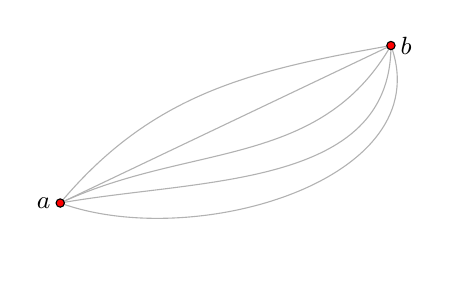
\begin{tikzpicture}
    \coordinate (a) at (0,0);
    \coordinate (b) at (4.2,2);
    % Líneas
    \draw[black!30] (a) to[out=50,in=190] (b);
    \draw[black!30] (a) -- (b);
    \draw[black!30] (a) to[out=25,in=-120] (b);
    \draw[black!30] (a) to[out=10,in=-90] (b);
    \draw[black!30] (a) to[out=-20,in=-70] (b);
    % Puntos
    \fill[fill=red,draw=black] (a) circle[radius=1.5pt] node[left] {\small $a$};
    \fill[fill=red,draw=black] (b) circle[radius=1.5pt] node[right] {\small $b$};
  \end{tikzpicture}
  \caption{Se aprecian algunas de las infinitas trayectorias posibles
    en dos dimensiones, entre los puntos $a$ y $b$ y los instantes
    $t_a$ y $t_b$.}
  \label{fig:infinitas_trayectorias}
\end{minipage}
% \hfil
\hspace{2em}
\begin{minipage}{0.50\linewidth}
  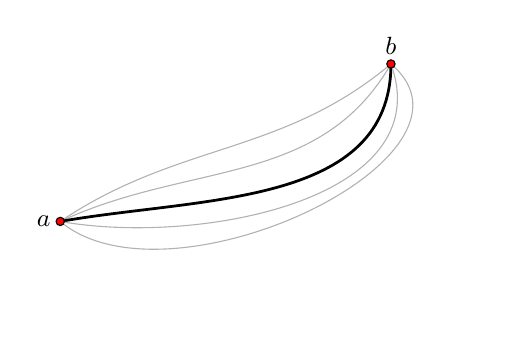
\begin{tikzpicture}
    \coordinate (a) at (0,0);
    \coordinate (b) at (4.2,2);
    % Líneas
    %\draw[black!30!white] (a) to[out=50,in=190] (b);
    %\draw[black!30!white] (a) -- (b);
    \draw[black!30] (a) to[out=34,in=-140] (b);
    \draw[black!30] (a) to[out=25,in=-120] (b);
    \draw[black,line width=1pt] (a) to[out=10,in=-90] (b);
    \draw[black!30] (a) to[out=-10,in=-70] (b);
    \draw[black!30] (a) to[out=-40,in=-40] (b);
    %\draw[black!30!white] (a) to[out=-20,in=-70] (b);
    % Puntos
    \fill[fill=red,draw=black] (a) circle[radius=1.5pt] node[left] {\small $a$};
    \fill[fill=red,draw=black] (b) circle[radius=1.5pt] node[above] {\small $b$};
  \end{tikzpicture}
  \caption{Podríamos calcular la acción $S$ asociada a cada
    trayectoria. La real, aquí en negro, será la que tenga la menor acción de entre
    las infinitas trayectorias posibles.}
  \label{fig:infinitas_trayectorias_y_la_real}
  \end{minipage}
\end{figure}

Para cada trayectoria, definida mediante la función $x=x(t)$, podemos
definir una magnitud conocida como \emph{la acción} asociada a la
trayectoria, $S[x(t)]$ o simplemente $S[x]$, como la integral entre
los dos intantes de tiempo, del lagrangiano de la partícula
\[
  S[x(t)] = S[x] = \int_{t_a}^{t_b} \mathcal{L}(x,\dot{x})\,dt
\]
Recuérdese que aquí $x$ no es una posición en un instante, sino una
función del tiempo. La acción, $S[x]$, es un \emph{funcional}, puesto
que es una función que asigna a una función, un valor real.

Tenemos que paremetrizar las infinitas trayectorias posibles entre los
puntos $a$ y $b$ en los instantes $t_a$ y $t_b$.  Para ello
consideraremos todas las posibles trayectorias que, partiendo de $a$
en el instante $t_a$, lleguen exactamente al punto $b$ en el instante
$t_b$. Es clave, en algún momento del desarrollo, darse cuenta de que
las infinitas trayectorias posibles tienen el mismo valor en los
extremos $a$ y $b$.

El \emph{principio de mínima acción} nos dice que la trayectoria real
será la que tenga menor acción.  Entonces, vamos a considerar la
trayectoria real (clásica), como la representada en negro en la
figura~\ref{fig:infinitas_trayectorias_y_la_real}, y pequeñísimas
variaciones de ésta, que como hemos comentado, tienen el mismo valor
en los extremos $a$ y $b$.

Las demás trayectorias se diferenciarán por muy poco de la real, la variación
en la acción es
\[
  \delta S = \int_{t_a}^{t_b}\delta\mathcal{L}(x,\dot{x})\,dt
\]

Por otro lado, como las trayectorias que consideramos están muy
próximas a la real, podemos desarrollar $\delta\mathcal{L}$ en
potencias de $x$ y $\dot{x}$, y despreciar los términos de segundo
orden en adelante
\[
  \delta\mathcal{L}(x,\dot{x})
  =
  \delta x\kern1pt\dfrac{\partial\mathcal{L}}{\partial x}
  +
  \delta\dot{x}\kern1pt\dfrac{\partial\mathcal{L}}{\partial\dot{x}}
\]

Así
\[
  \delta S
  =
  \int_{t_a}^{t_b} \left\{
    \delta x\kern1pt\dfrac{\partial\mathcal{L}}{\partial x}
    + \delta\dot{x}\kern1pt\dfrac{\partial\mathcal{L}}{\partial\dot{x}}
  \right\}\,dt
  =
  \int_{t_a}^{t_b} 
    \delta x\kern1pt\dfrac{\partial\mathcal{L}}{\partial x}\,dt
    +
    \int_{t_a}^{t_b} \delta\dot{x}\kern1pt\dfrac{\partial\mathcal{L}}{\partial\dot{x}}\,dt
\]

Resolvemos la segunda integral por partes

\smallskip
\begin{center}
\begin{tabular}{lcl}
  $u = \dfrac{\partial\mathcal{L}}{\partial\dot{x}}$
  &$\longrightarrow$
  &$du = \dfrac{d}{dt} \left(\dfrac{\partial\mathcal{L}}{\partial\dot{x}}\right)$\\
  $dv = \delta\dot{x}\,dt$
  &$\longrightarrow$
  &$v=\delta x$
\end{tabular}
\end{center}

\[
  \int_{t_a}^{t_b}
  \delta\dot{x}\kern1pt\dfrac{\partial\mathcal{L}}{\partial\dot{x}}\,dt
  = \left[\delta x \dfrac{\partial\mathcal{L}}{\partial\dot{x}}\right]_{t_a}^{t_b}
  - \int_{t_a}^{t_b}
  \delta x\,\dfrac{d}{dt} \left(\dfrac{\partial\mathcal{L}}{\partial\dot{x}}\right)\,dt
  =
  - \int_{t_a}^{t_b}
  \delta x\,\dfrac{d}{dt} \left(\dfrac{\partial\mathcal{L}}{\partial\dot{x}}\right)\,dt
\]
El primer término es cero porque implica calcular $\delta
x$ en los puntos, $t_a$ y
$t_b$, que vale cero, porque la infinita familia de funciones valen lo
mismo en $t_a$ y $t_b$.

La variación de la acción queda
\[
  \delta S
  =
  \int_{t_a}^{t_b} \delta x\,\dfrac{\partial\mathcal{L}}{\partial x}\,dt
  - \int_{t_a}^{t_b}
  \delta x\,\dfrac{d}{dt} \left(\dfrac{\partial\mathcal{L}}{\partial\dot{x}}\right)\,dt
  =
  \int_{t_a}^{t_b} \delta x\,
  \left\{\dfrac{\partial\mathcal{L}}{\partial x}
  - \dfrac{d}{dt} \left(\dfrac{\partial\mathcal{L}}{\partial\dot{x}}\right)\right\}\,dt
\]

La variación del funcional, $S$, con respecto a la trayectoria $x$
\[
  \dfrac{\delta S}{\delta x}
  =
  \int_{t_a}^{t_b} 
  \left\{\dfrac{\partial\mathcal{L}}{\partial x}
  - \dfrac{d}{dt} \left(\dfrac{\partial\mathcal{L}}{\partial\dot{x}}\right)\right\}\,dt
\]

La igualamos a cero
\[
    \dfrac{\delta S}{\delta x}
  =
  \int_{t_a}^{t_b} 
  \left\{\dfrac{\partial\mathcal{L}}{\partial x}
    - \dfrac{d}{dt} \left(\dfrac{\partial\mathcal{L}}{\partial\dot{x}}\right)\right\}\,dt
  = 0
\]

Y queda la ecuación de Euler-Lagrange para la partícula en una
dimensión, de la que podremos obtener la trayectoria real
\[
  \dfrac{\partial\mathcal{L}}{\partial x}
    = \dfrac{d}{dt} \left(\dfrac{\partial\mathcal{L}}{\partial\dot{x}}\right)
\]

\subsection{Acción clásica de una partícula libre}

Seguimos con el tratamiento clásico. La acción para una partícula en
una dimensión se define como
\[
  S
  =
  \int_{t_a}^{t_b} \mathcal{L}(x, \dot{x})\,dt
\]

El lagrangiano de una partícula libre es
\[
  \mathcal{L}(x,\dot{x})
  =
  T - U
  =
  \dfrac{1}{2}m\dot{x}^2 - 0
  =
  \dfrac{1}{2}m\dot{x}^2
\]

Calculamos las derivadas necesarias
\[
  \dfrac{\partial\mathcal{L}}{\partial x}
  =
  0
  \hspace{2em}\text{y}\hspace{2em}
  \dfrac{d}{dt}\left(\dfrac{\partial\mathcal{L}}{\partial\dot{x}}\right)
    =
    \dfrac{d}{dt} (m\dot{x})
\]

Aplicando la ecuación de Euler-Lagrange, comprobamos que la partícula
tiene velocidad constante
\[
  \dfrac{d}{dt} (m\dot{x}) = 0
  ;\hspace{1em}
  \dot{x} = \text{ constante}
\]

La mínima acción se obtendrá cuando $\dot{x}$ sea constante
\begin{align*}
  S^{\textsc{cl}}
  &=
  \int_{t_a}^{t_b} \dfrac{1}{2} m\dot{x}^2\,dt
  =
  \dfrac{1}{2} m\dot{x}^2 \int_{t_a}^{t_b} dt
  =
  \dfrac{1}{2}m\dot{x}^2 (t_b-t_a)
  =
    \dfrac{1}{2}m \dfrac{(x_b-x_a)^2}{(t_b-t_a)^{\cancelout{\scriptstyle 2}}}\kern1pt \cancelout{(t_b-t_a)}\\
  &= \dfrac{m\kern1pt (x_b-x_a)^2}{2\kern1pt (t_b-t_a)}
\end{align*}

La acción para una partícula clásica libre es
\begin{equation}\label{eq:accion_clasica_particula_libre}
  S^{\textsc{cl}}
  =
  \dfrac{m\kern1pt (x_b-x_a)^2}{2\kern1pt (t_b-t_a)}
  =
  \dfrac{p^2}{2m}\kern1pt (t_b-t_a)
\end{equation}

\subsection{Acción clásica de un oscilador armónico}
Nos proponemos obtener la acción clásica de un oscilador armónico. Para ello, mediante la ecuación de Euler-Lagrange obtendremos la ecuación diferencial del movimiento, después la resolveremos y por último calcularemos la acción correspondiente a esa trayectoria.

\subsubsection{Ecuación de Euler-Lagrange}
El lagrangiano de un oscilador armónico es
\[
  \mathcal{L}(x,\dot{x})
  =
  \dfrac{1}{2}m\dot{x}^2
  -
  \dfrac{1}{2}kx^2
\]

Calculamos las derivadas del lagrangiano
\begin{align*}
  &\dfrac{\partial\mathcal{L}}{\partial x}
  =
    -kx\\
  &\dfrac{d}{dt}\left(\dfrac{\partial\mathcal{L}}{\partial\dot{x}}\right)
  =
  \dfrac{d}{dt}m\dot{x}
  =
  m\ddot{x}
\end{align*}

La solución de la ecuación de Euler-Lagrange nos da la trayectoria
real del oscilador armónico, esto es, la que tiene la menor acción
\[
  \dfrac{\partial\mathcal{L}}{\partial x}
  =
  \dfrac{d}{dt}\left(\dfrac{\mathcal{L}}{\partial\dot{x}}\right)
\]

Sustituyendo las derivadas en la ecuación anterior, obtenemos
\[
  -kx = m\ddot{x}
\]
que es una ecuación diferencial de segundo orden, de coeficientes
constantes y homogénea
\[
  m\ddot{x}+kx = 0
\]

\subsubsection{Solución de la ecuación diferencial}
Ahora queremos resolver la ecuación diferencial para obtener la
trayectoria clásica (de menor acción) del oscilador armónico.

Probamos una solución del tipo $x(t)=e^{st}$
\[
  x = e^{st}
  ;\hspace{1em}
  \dot{x} = se^{st}
  ;\hspace{1em}
  \ddot{x} = s^2e^{st}
\]

Sustituimos en la ecuación diferencial y obtenemos la ecuación característica
\[
  m s^2e^{st} + ke^{st} = 0
  ;\hspace{1em}
  ms^2 + k = 0
\]
De ella deducimos el valor de $s$
\[
  s^2 = -\dfrac{k}{m}
  ;\hspace{1em}
  s = \pm i\kern1pt\sqrt{\dfrac{k}{m}}
  = \pm i\omega
\]
Donde hemos llamado $\omega$, la frecuencia natural del oscilador, a $\sqrt{k/m}$.

La solución general de la ecuación de Euler-Lagrange será
\begin{align*}
  x(t)
  &= x = c_1 e^{i\omega t} + c_2 e^{-i\omega t}
  = c_1(\cos\omega t + i\sin\omega t) + c_2(\cos(-\omega t) + i\sin(-\omega t))\\
  &=
    c_1(\cos\omega t + i\sin\omega t) + c_2(\cos\omega t - i\sin\omega t)
    = (c_1+c_2) \cos\omega t + i (c_1-c_2) \sin\omega t\\
    &= A \cos\omega t + B\sin\omega t
\end{align*}

\subsubsection{Expresión de la solución en función de $x_a$, $t_a$,
  $x_b$ y $t_b$}
Una vez obtenida la trayectoria clásica hemos de expresar las
constantes de integración $A$ y $B$ en función de las variables de los puntos extremos de la trayectoria $x_a$, $t_a$, $x_b$ y $t_b$.

Sabemos que $x_a=x(t_a)$ y $x_b=x(t_b)$
\begin{align*}
  x_a &= A\cos\omega t_a + B\sin\omega t_a\\
  x_b &= A\cos\omega t_b + B\sin\omega t_b
\end{align*}

Su expresión matricial es
\[
  \begin{pmatrix} x_a \\ x_b \end{pmatrix}
  =
  \begin{pmatrix}
    \cos\omega t_a & \sin\omega t_a\\
    \cos\omega t_b & \sin\omega t_b
  \end{pmatrix}
  \begin{pmatrix} A \\ B \end{pmatrix}
\]

Podemos ahora calcular $A$ y $B$ en función de las posiciones y
tiempos en los extremos, mediante la matriz inversa
\begin{align*}
  \begin{pmatrix} A \\ B \end{pmatrix}
  &=
  \begin{pmatrix}
    \cos\omega t_a & \sin\omega t_a\\
    \cos\omega t_b & \sin\omega t_b
  \end{pmatrix}^{-1}
  \begin{pmatrix} x_a \\ x_b \end{pmatrix}
  =
  \dfrac{1}{\sin\omega(t_b-t_a)}
  \begin{pmatrix}
    \sin\omega t_b & -\sin\omega t_a\\
    -\cos\omega t_b & \cos\omega t_a
  \end{pmatrix}
  \begin{pmatrix} x_a \\ x_b \end{pmatrix}\\
  &=
    \dfrac{1}{\sin\omega(t_b-t_a)}
    \begin{pmatrix}
      x_a\sin\omega t_b - x_b\sin\omega t_a \\
      -x_a\cos\omega t_b + x_b\cos\omega t_a
    \end{pmatrix}
\end{align*}

Las constantes valen
\begin{align*}
  A &= \dfrac{x_a\sin\omega t_b-x_b\sin\omega t_a}{\sin\omega(t_b-t_a)}\\
  B &= \dfrac{-x_a\cos\omega t_b+x_b\cos\omega t_a}{\sin\omega(t_b-t_a)}
  \end{align*}

  \subsubsection{Trayectoria clásica en función de $x_a$, $t_a$, $x_b$ y $t_b$}

  La trayectoria clásica es
  \begin{align*}
    x
    &=
    \dfrac{x_a\sin\omega t_b-x_b\sin\omega t_a}{\sin\omega(t_b-t_a)} \cos\omega t
    +
    \dfrac{-x_a\cos\omega t_b+x_b\cos\omega t_a}{\sin\omega(t_b-t_a)} \sin\omega t\\
    &=
        \dfrac{x_a(\sin\omega t_b\cos\omega t-\cos\omega t \sin\omega t_a)
        + x_b(\sin\omega t \cos\omega t_a - \cos\omega t \sin\omega t_a)}
        {\sin\omega(t_b-t_a)}\\
    &=
      \dfrac{x_a\sin\omega (t_b-t) + x_b\sin\omega (t-t_a)}{\sin\omega(t_b-t_a)}
  \end{align*}

  La velocidad es
\begin{align*}
  \dot{x}
    &=
      \dfrac{-x_a\omega\cos\omega (t_b-t) + x_b\omega\cos\omega (t-t_a)}{\sin\omega(t_b-t_a)}
\end{align*}
  
\subsubsection{Acción clásica del oscilador armónico}
Primero calculamos las expresiones $\omega^2x²$ y $\dot{x}^2$ que
aparecerán en el cálculo de la acción
\begin{align*}
  \omega^2x^2
  &=
    \omega^2\,
    \dfrac{x_a^2\sin^2\omega(t_b-t)+x_b^2\sin^2\omega(t-t_a)+2x_ax_b\sin\omega(t_b-t)\sin\omega(t-t_a)}
    {\sin^2\omega(t_b-t_a)}
  %&=
   % \omega^2\,
   % \dfrac{x_a^2\sin^2\omega(t_b-t)+x_b^2\sin^2\omega(t-t_a)+2x_ax_b\sin\omega(t_b-t)\sin\omega(t-t_a)}
  %{\sin^2\omega D}\\
  \end{align*}
  
\begin{align*}
  \dot{x}^2
  &=
    \omega^2\,
    \dfrac{x_a^2\cos^2\omega(t_b-t)+x_b^2\cos^2\omega(t-t_a)-2x_ax_b\cos\omega(t_b-t)\cos\omega(t-t_a)}
    {\sin^2\omega(t_b-t_a)}
\end{align*}

La acción clásica se obtiene sustituyendo en el lagrangiano la
trayectoria clásica (y su derivada) obtenida anteriormente
\begin{align*}
   S^{\textsc{cl}}
   &=
   \int_{t_a}^{t_b}\mathcal{L}(x,\dot{x})\,dt
   =
   \int_{t_a}^{t_b}\left(\dfrac{1}{2}m\dot{x}^2-\dfrac{1}{2}m\omega^2x^2\right)\,dt
   = \dfrac{m}{2} \int_{t_a}^{t_b}(\dot{x}^2 - \omega^2 x^2)\,dt
 \end{align*}

 Sustituimos en la acción, con ayuda de las expresiones anteriores y
 la escribimos en función del coseno del ángulo doble,
 $\cos 2a = \cos^2a-\sin^2a$
 {\small
 \[
    S^{\textsc{cl}}
    =
      \dfrac{m\omega^2}{2\sin^2\omega(t_b-t_a)}\int_{t_a}^{t_b}
      [x_a^2\cos 2\omega(t_b-t) + x_b^2\cos 2\omega(t-t_a)
      -2x_ax_b\cos(2\omega t-\omega(t_a+t_b))]\,dt
 \]
}

La acción queda en función de una integral, $I$, que resolveremos
aparte
\begin{equation}\label{eq:oscilador_armonico_accion_clasica_I}
  S^{\textsc{cl}} = \dfrac{m\omega^2}{2\sin^2\omega(t_b-t_a)}\,I
\end{equation}

{\small
\begin{align*}
 I
  &=
    \int_{t_a}^{t_b}
    [x_a^2\cos 2\omega(t_b-t) + x_b^2\cos 2\omega(t-t_a)
    -2x_ax_b\cos(2\omega t-\omega(t_a+t_b))]\,dt\\
  &=
    x_a^2\int_{t_a}^{t_b}\cos 2\omega(t_b-t)\,dt
    + x_b^2\int_{t_a}^{t_b}\cos 2\omega(t-t_a)\,dt
    -2x_ax_b\int_{t_a}^{t_b}\cos(2\omega t-\omega(t_a+t_b))\,dt
\end{align*}
}

Las dos primeras integrales tienen el mismo valor
\begin{align*}
  I
  &=
    x_a^2\,\dfrac{\sin 2\omega(t_b-t_a)}{2\omega}
    + x_b^2\,\dfrac{\sin 2\omega(t_b-t_a)}{2\omega}
    - 2x_ax_b\,\dfrac{\sin\omega(t_b-t_a)}{\omega}\\
  &=
    \dfrac{1}{\omega} \left[(x_a^2+x_b^2)\,\dfrac{\sin 2\omega(t_b-t_a)}{2}
    - 2x_ax_b\,\sin\omega(t_b-t_a)\right]\\
  &=
    \dfrac{1}{\omega} \left[(x_a^2+x_b^2)\,\dfrac{\cancelout{2}\sin\omega(t_b-t_a) \cos\omega(t_b-t_a)}{\cancelout{2}}
    - 2x_ax_b\,\sin\omega(t_b-t_a)\right]\\
  &=
    \dfrac{\sin\omega(t_b-t_a)}{\omega}
    \left[(x_a^2+x_b^2)\,\cos\omega(t_b-t_a) - 2x_ax_b\right]
\end{align*}

Sustituimos este resultado en la acción clásica,
ecuación~(\ref{eq:oscilador_armonico_accion_clasica_I})
\[
  S^{\textsc{cl}}
  =
  \dfrac{m\omega^{\cancelout{\scriptstyle 2}}}
  {2\sin^{\cancelout{\scriptstyle 2}}\omega(t_b-t_a)}\,
    \dfrac{\cancelout{\sin\omega(t_b-t_a)}}{\cancelout{\omega}}
    \left[(x_a^2+x_b^2)\,\cos\omega(t_b-t_a) - 2x_ax_b\right]
\]

Quedando, por fin, la acción clásica de un oscilador armónico
\begin{equation}\label{eq:oscilador_armonico_accion_clasica}
  S^{\textsc{cl}}
  =
  \dfrac{m\omega}
  {2\sin\omega(t_b-t_a)}\,
  \left[(x_a^2+x_b^2)\,\cos\omega(t_b-t_a) - 2x_ax_b\right]
\end{equation}

\section{Ondas de materia}
A principios del siglo XX se sabía que la luz tenía un doble
comportamiento onda-corpúsculo. Por un lado se podía considerar como
una onda, caracterizada por una frecuencia y una longitud de onda, y
por otro, se podía considerar formada por partículas sin masa
denominadas fotones. Podemos resumir este doble comportamiento
mediante las ecuaciones
\begin{align*}
  E &= \hslash\omega\\
  p &= \dfrac{\Planckconst}{\lambda} = \hslash k
\end{align*}

donde $E$ es la energía de un fotón, $\omega$ es la frecuencia angular
de la luz, $p$ es su momento lineal, $k$ es el número de ondas y
$\hslash$ es la constante de Planck reducida.

De Broglie sugirió que las partículas podrían tener también este doble
comportamiento. Para una+ partícula libre
\begin{align}\label{eq:DeBroglie_energia}
  E &= \dfrac{p^2}{2m} = \hslash\omega\\
  \label{eq:DeBroglie_momento_lineal}
  p &= \hslash k = \dfrac{\Planckconst}{\lambda}
\end{align}

La ecuación genérica de una onda de una sola frecuencia se puede
escribir en forma compleja, como
\[
  \phi (x,t)
  =
  A e^{i(kx-\omega t)}
\]
donde $A$ representa la amplitud.

Para una partícula libre, según De Broglie,
ecuaciones~(\ref{eq:DeBroglie_energia})
y~(\ref{eq:DeBroglie_momento_lineal})
\[
  \omega = \dfrac{p^2}{2m\hslash}
  \hspace{1em}\text{y}\hspace{1em}
  k = \dfrac{p}{\hslash}
\]
\[
  \phi (x,t)
  =
  A \exp\left[i\left(\dfrac{p}{\hslash}x-\dfrac{p^2}{2m\hslash}t\right)\right]
    =
  A \exp\left[\dfrac{i}{\hslash}\left(px-\dfrac{p^2}{2m}t\right)\right]
\]

La onda compleja sería
\[
  \phi (x,t)
  =
  A e^{i\theta}
  ;\hspace{1em}
  \theta = \dfrac{p}{\hslash} x - \dfrac{p^2}{2m\hslash}t 
\]

Estamos interesados en el cambio de ángulo de fase el tiempo $t_a$ y posición $x_a$ hasta $t_b$ y $x_b$.
\begin{figure}[ht]
  %\centering
  \begin{minipage}{0.58\linewidth}
    \centering
    \begin{tikzpicture}
      \def\posA{0.5}
      \def\posB{4.5}
      \coordinate (origen) at (0,0);
      \coordinate (xa) at (\posA,0);
      \coordinate (xb) at (\posB,0);
      \newcommand{\colorAng}{green!60}
      \newcommand{\colorAngLin}{green!30!black}
      
      % Línea horizontal gris claro
      \draw[ultra thin,black!20] (-1,0) -- (6,0) coordinate (eje x);

      % Primer complejo
      \fill[fill=black,draw=black!20] (\posA,0) circle[radius=1.5pt]
      coordinate (xa) node[below=2pt]{\small$x_a$} node[below=11pt]
      {\small$t_a$};
      \draw[-{Latex},line width=1pt,black] (\posA,0) -- +(30:1.5)
      coordinate (v1) node[above] {$\phi_a$};
      \path (eje x) -- (xa) -- (v1) pic
      [draw=\colorAngLin,fill=\colorAng,-{Latex[length=1.3mm,scale=0.80,bend]},
      "\footnotesize$\theta_a$",angle radius=5mm,angle eccentricity=1.5]
      {angle = eje x--xa--v1};
      \fill[fill=black,draw=black!20] (\posA,0) circle[radius=1.5pt]
      node[below=2pt]{\small$x_a$} node[below=11pt]
      {\small$t_a$};
      
    % Segundo complejo
      \draw[-{Latex},line width=1pt,black] (\posB,0) -- +(115:1.5)
      coordinate (v2) node[left] {$\phi_b$};
      \path (eje x) -- (xb) -- (v2) pic
      [draw=\colorAngLin,fill=\colorAng,-{Latex[length=1.3mm,scale=0.80,bend]},
      "\footnotesize$\theta_b$",angle radius=5mm,angle eccentricity=1.5]
      {angle = eje x--xb--v2};
      \fill[fill=black,draw=black!20] (\posB,0) circle[radius=1.5pt]
      node[below=2pt]{\small$x_b$} node[below=11pt]
      {\small$t_b$};
  \end{tikzpicture}
  \caption{Al avanzar la onda, el ángulo de fase va cambiando. Aquí
    avanza de izquierda a derecha, esto es $t_a<t_b$.}
\end{minipage}
\hspace{3em}
\begin{minipage}{0.3\linewidth}
  \centering
  \begin{tikzpicture}
      \def\posV{0.5}
      \coordinate (origen) at (\posV,0);
      \newcommand{\colorAng}{orange!50}
      \newcommand{\colorAngLin}{black}

    % Línea horizontal gris claro
    \draw[-{Latex},line width=1pt,black] (origen) -- +(115:1.5) coordinate (v2)
    node[left] {$\phi_b$};
    \draw[-{Latex},line width=1pt,black] (origen) -- +(30:1.5) coordinate (v1)
    node[right] {$\phi_a$};
    \path (v1) -- (origen) -- (v2) pic
    [draw=black!60,fill=\colorAng,-{Latex[length=1.3mm,scale=0.80,bend]},
    "\footnotesize$\Delta\theta$",angle radius=5mm,angle eccentricity=1.5]
    {angle = v1--origen--v2};
    \fill[fill=black,draw=black!20] (origen) circle[radius=1.5pt]
    node[below=11pt] {\small$\phantom{t_b}$};
  \end{tikzpicture}
  \caption{El ángulo girado entre $t_a$ y $t_b$, en los puntos $x_a$ y
    $x_b$ es $\Delta\theta$.}
\end{minipage}
\end{figure}

Calculamos el incremento de $\hslash\theta$ cuando una onda material
pasa de $x_a$ en un instante $t_a$ a otra $x_b$ en el instante $t_b$
\begin{align*}
  \hslash\Delta\theta
  &=
  \hslash\theta_b - \hslash\theta_a
  =
  \left(p\kern1pt x_b-\dfrac{p^2}{2m}\kern1pt t_b\right)
  -
  \left(p\kern1pt x_a-\dfrac{p^2}{2m}\kern1pt t_a\right)
  =
    p\kern1pt (x_b-x_a)-\dfrac{p^2}{2m}\kern1pt (t_b-t_a)\\
  &=
    m\kern1pt\dfrac{x_b-x_a}{t_b-t_a}\kern1pt (x_b-x_a)
    -
    \dfrac{m^{\cancelout{\scriptstyle 2}}(x_b-x_a)^2/(t_b-t_a)^{\cancelout{\scriptstyle 2}}}{2\cancelout{m}}
    \cancelout{(t_b-t_a)}\\
  &=
    \dfrac{m\kern1pt(x_b-x_a)^2}{2\kern1pt(t_b-t_a)}
    =
    \dfrac{p^2}{2m}\kern1pt (t_b-t_a)
    = S^{CL}
\end{align*}

Éste último término es la acción clásica de una partícula libre,
ecuación~(\ref{eq:accion_clasica_particula_libre}).

Así, la onda de materia queda
\[
  \phi (x,t) = A e^{i S^{\textsc{cl}}/\hslash}
  = A\exp\left\{\dfrac{i}{\hslash}\dfrac{m(x_b-x_a)^2}{2(t_b-t_a)}\right\}
\]

Fue esta relación, entre una onda de materia y la acción, la que llevó
a Feynman a introducir una nueva formulación de la mecánica cuántica.

\subsection{Postulados de la mecánica cuántica}
Presentamos de una forma sencilla algunos postulados de la
formulación de Feynman de la mecánica cuántica
\begin{enumerate}
\item Existe un número complejo, $\phi$, para cada proceso. Este
  número se denomina amplitud de probabilidad.
\item Si hay varias maneras de conectar el inicio y el fin de un
  proceso, $\phi_1$, $\phi_2$, $\cdots$, entonces la amplitud de ese
  proceso es la suma
  \[
    \phi = \phi_1 + \phi_2 + \cdots
  \]

\item La probabilidad de que ocurra el proceso es el cuadrado del complejo
  \[
    P = |\phi|^2 = \phi^* \phi = |\phi_1 + \phi_2 + \cdots|^2
  \]

\item La estructura de cada amplitud, $\phi_i$ es
  \[
    \phi_i = A e^{i S/\hslash}
  \]

  donde $A$ depende de la acción.
\end{enumerate}

\subsection{Desarrollo de la acción hasta segundo orden}
Queremos obtener una expresión para la acción de un sistema, mediante
un desarrollo en serie del lagrangiano hasta segundo orden.

Supondremos una partícula sujeta a un potencial $U(x)$, que se
mueve en una dimensión. Su lagrangiano es
\[
  \mathcal{L}(x,\dot{x})
  =
  \dfrac{1}{2}m\dot{x}^2 - U(x)
\]
donde $x$ representa una cierta trayectoria $x=x(t)$ y $\dot{x}$ la
velocidad en cada punto de la misma, $\dot{x}=\dot{x}(t)$.

Tomamos como referencia una trayectoria en particular, por ejemplo la
clásica, y consideramos pequeñas variaciones, $z$, con respecto a
ésta, $x = x^{\textsc{cl}} + z$ (ver
figura~\ref{fig:trayectoria_clasica_pequeñas_variaciones})

\begin{figure}[ht]
  \centering
  \begin{tikzpicture}
    \coordinate (a) at (0,0);
    \coordinate (b) at (4.2,2);
    % Líneas
    \draw[black!30!white,name path=var] (a) to[out=25,in=-129] (b);
    \draw[black,line width=1pt,name path=cla]
    (a)  to[out=10,in=-90] node[below] {$x^{\text{\textsc{cl}}}$} (b);
    \path[name path=vertical] (3.3,0) -- +(up:2); 
    % Intersecciones
    \path[name intersections={of=cla and vertical}]
    (intersection-1) coordinate (p1);
    \path[name intersections={of=var and vertical}]
    (intersection-1) coordinate (p2);
    % z
    \draw[-{Latex[round,length=4pt]},green!50!black]
    (p1) -- node[right,pos=0.6] {$z$} (p2);
    % Puntos
    \fill[fill=red,draw=black] (a) circle[radius=1.5pt] node[left] {\small $a$};
    \fill[fill=red,draw=black] (b) circle[radius=1.5pt] node[above] {\small $b$};
  \end{tikzpicture}
  \caption{Consideramos pequeñas variaciones, $z$, de la trayectoria
    clásica, $x=x^{\textsc{cl}}+z$ }
  \label{fig:trayectoria_clasica_pequeñas_variaciones}
\end{figure}

Desarrollamos el lagrangiano en serie de potencias de $z$ y $\dot{z}$, hasta segundo orden
\begin{align*}
  \mathcal{L}{x,\dot{x}}
  &=
  \mathcal{L}(x^{\textsc{cl}}+z,\dot{x}^{\textsc{cl}}+\dot{z})\\
  &= 
  \mathcal{L}(x^{\textsc{cl}},\dot{x}^{\textsc{cl}})
  + z\,\dfrac{\partial\mathcal{L}}{\partial z}
  + \dot{z}\kern1pt\dfrac{\partial\mathcal{L}}{\partial\dot{z}}
  + \dfrac{1}{2} z^2 \kern1pt\dfrac{\partial^2\mathcal{L}}{\partial z^2}
  + z \dot{z}\kern1pt \dfrac{\partial^2\mathcal{L}}{\partial z\partial\dot{z}}
  + \dfrac{1}{2} \dot{z}^2 \kern1pt\dfrac{\partial^2\mathcal{L}}{\partial\dot{z}^2}
\end{align*}

Calculamos las derivadas parciales
\begin{align*}
  &\dfrac{\partial\mathcal{L}}{\partial z}
  = \dfrac{\partial\mathcal{L}}{\partial x}\cdot\dfrac{dx}{dz}
    = -U'(x)\cdot 1 = -U'(x)\\
  &\dfrac{\partial^2\mathcal{L}}{\partial z^2}
    = \dfrac{\partial}{\partial z} \left(\dfrac{\partial\mathcal{L}}{\partial z}\right)
    = \dfrac{\partial}{\partial z} \left(-U'(x)\right)
    = \dfrac{\partial (-U'(x))}{\partial x}\cdot\dfrac{dz}{dx}
    = -U''(x)\cdot 1
    = -U''(x)\\
  &\dfrac{\partial\mathcal{L}}{\partial\dot{z}}
  = \dfrac{\partial\mathcal{L}}{\partial\dot{x}}\cdot\dfrac{d\dot{x}}{d\dot{z}}
    = m\dot{x}\cdot 1 = m\dot{x}\\
  &\dfrac{\partial^2\mathcal{L}}{\partial \dot{z}^2}
    = \dfrac{\partial}{\partial\dot{z}} \left(\dfrac{\partial\mathcal{L}}{\partial\dot{z}}\right)
    = \dfrac{\partial}{\partial\dot{z}}\left(m\dot{x}\right)
    = \dfrac{\partial (m\dot{x})}{\partial\dot{x}}\cdot\dfrac{d\dot{x}}{d\dot{z}}
    = m\cdot 1
    = m\\
  &\dfrac{\partial^2\mathcal{L}}{\partial\dot{z} \partial z}
    = \dfrac{\partial^2\mathcal{L}}{\partial z \partial\dot{z}}
    = \dfrac{\partial}{\partial z} \left(\dfrac{\partial\mathcal{L}}{\partial\dot{z}}\right)
    = \dfrac{\partial}{\partial z}\left(m\dot{x}\right)
    = \dfrac{\partial (m\dot{x})}{\partial x}\cdot\dfrac{d x}{d z}
    = 0\cdot 1
    = 0
\end{align*}

El lagrangiano (hasta segundo orden) queda
\[
  \mathcal{L}(x^{\textsc{cl}}+z,\dot{x}^{\textsc{cl}}+\dot{z})
  \approx
  \mathcal{L}(x^{\textsc{cl}},\dot{x}^{\textsc{cl}})
  - z U'(x)
  + m\dot{x}\dot{z}
  - \dfrac{1}{2}z^2 U''(x)
  + \dfrac{1}{2}m\dot{z}^2
\]

La acción correspondiente será
\[
  S[x^{\textsc{cl}}+z]
  \approx
  \int_{t_a}^{t_b}
  \left[
    \mathcal{L}(x^{\textsc{cl}},\dot{x}^{\textsc{cl}})
  - z U'(x)
  + m\dot{x}\dot{z}
  - \dfrac{1}{2}z^2 U''(x)
  + \dfrac{1}{2}m\dot{z}^2
  \right]\,dt
\]

Calculamos aparte la integral del tercer sumando aplicando partes
\begin{center}
  \begin{tabular}{lcl}
    $u=m\dot{x}$
    &\hspace{1em}$\longrightarrow$\hspace{1em}
    &$du=m\ddot{x}$\\
    $dv=\dot{z}\,dt$
    &\hspace{1em}$\longrightarrow$\hspace{1em}
    &$v=z$
  \end{tabular}
\end{center}

\[
  \int_{t_a}^{t_b} m\dot{x}\dot{z}\,dt
  =
  \left[m\dot{z} z\right]_{t_a}^{t_b}
  - \int_{t_a}^{t_b} m\ddot{x} z\,dt
  =
  - \int_{t_a}^{t_b} m\ddot{x} z\,dt
\]
El primer término de la integral se anula porque implica el cálculo de
$\Delta x$ en los puntos extremos $t_a$ y $t_b$, que vale cero en
ambos.

La acción queda
\begin{align*}
  S[x^{\textsc{cl}}+z]
  &=
    S[x^{\textsc{cl}}]
    - \int_{t_a}^{t_b}\left[\cancelout{U'(x)+m\ddot{x}}\right] z\,dt
    + \int_{t_a}^{t_b}\left[\dfrac{1}{2}m\dot{z}^2-\dfrac{1}{2}z^2 U''(x)\right]\,dt
\end{align*}

El segundo sumando de la expresión anterior se anula porque la fuerza
es menos la derivada del potencial
\[
  m\ddot{x} = -U'(x)
\]

Finalmente, la acción para pequeñas variaciones de la trayectoria clásica
\begin{equation}\label{eq:accion_aprox_segundo_orden}
  S[x]
  =
  S[x^{\textsc{cl}}+z]
  \approx
  S[x^{\textsc{cl}}]
  + \int_{t_a}^{t_b}\left[\dfrac{1}{2}m\dot{z}^2-\dfrac{1}{2}z^2 U''(x)\right]\,dt
\end{equation}

\section{Integral de caminos de Feynman}
\subsection{Propagador de una partícula}
Supongamos que una partícula de masa $m$ se encuentra en el instante
$t_a$ en la posición $x_b$, y más tarde, en el instante $t_b$ se halla
en la posición $x_b$. Nos interesa hallar la amplitud de probabilidad
de que siga una trayectoria determinada ---llamémosla $j$---. Esta
trayectoria puede ser cualquiera, incluyendo las posiciones en
$x=-\infty$ y $x=\infty$; la única condición es que no viaje atrás en
el tiempo.

La amplitud de probabilidad $\phi_j$ de que la partícula siga esa
trayectoria $j$ es
\begin{align*}
  \phi_j
  &= A \exp\left\{\dfrac{i}{\hslash} S[x_j]\right\}
    = A \exp\left\{\frac{i}{\hslash} \int_{t_a}^{t_b} \mathcal{L}(x,\dot{x})\kern1pt dt\right\}\\
  &= A \exp\left\{\frac{i}{\hslash} \int_{t_a}^{t_b} \left(\dfrac{1}{2}m\dot{x}^2-U(x)\right)\kern1pt dt\right\}
\end{align*}
Nótese que aún no estamos considerando que la partícula sea libre,
debido a la presencia en la fórmula de la energía potencial de
interacción, $U(x)$.

Ahora queremos incluir todas las trayectorias posibles. Se llama
propagador de la partícula, $K(x_b,t_b;x_a,t_a)$ o, de forma
abreviada, $K(b;a)$, a la suma de todas las amplitudes de probabilidad
de todas las trayectorias posibles
\[
  K(x_b,t_b; x_a,t_a)
  =
  A \int_{-\infty}^{\infty} dx \exp\left\{\frac{i}{\hslash}\,\int_{t_a}^{t_b}\left(\frac{1}{2}m\dot{x}^2-U(x)\right)\kern1pt dt\right\}
\]

\subsection{Discretización del tiempo}
Por cuestiones prácticas, conviene discretizar el tiempo. Dividimos el
intervalo $t_b-t_a$ en $N$ tramos iguales, tal como se representa en
la figura~\ref{fig:path_integral_blank} ---cuanto mayor sea el valor
de $N$, más preciso será el cálculo---. Al final impondremos que $N$
tiende a infinito y eliminaremos la discretización. Llamamos
$\varepsilon$ a cada paso discreto en el eje del tiempo, esto es a la
distancia entre dos líneas horizontales consecutivas
\[
  \varepsilon = \dfrac{t_b-t_a}{N}
\]

Cada valor discreto de tiempo entre $t_a$ y $t_b$, según esta
partición, se calcula mediante
\[
  t_n = t_a + n\kern1pt\varepsilon
  ;\hspace{1em}
  n = 0, 1, 2, \cdots N
\]

\begin{figure}[ht]
  \centering
  \begin{minipage}{0.99\linewidth}
  \begin{tikzpicture}
    % Pequeñas marcas en los ejes para xa, xb, ta y tb
    \def\tick{.10}
    % Definiciones eje x
    \def\xorigen{0}
    \def\xmax{7.5}
    \def\xmin{-4.0}
    \def\xa{1}
    \def\xb{3.5}
    % Definiciones eje y
    \def\yorigen{0}
    \def\ymin{-0.5}
    \def\ymax{4.5}
    \def\ta{0.5}
    \def\tb{3.5}
    \def\partes{10}
    % Coordenadas
    \coordinate (origen) at (\xorigen,\yorigen);
    % Partición del tiempo
    \foreach \i in {0,1,...,\partes}
    \draw[{Straight Barb}-{Straight Barb},black!20,ultra thin] (\xmin,{\ta+\i*(\tb-\ta)/\partes}) -- (\xmax,{\ta+\i*(\tb-\ta)/\partes});

    \draw[-{>},ultra thin] (\xmin,\yorigen)
    -- (\xmax,\yorigen) coordinate (eje x) node[right]{\small $x$};
    \draw[-{>},ultra thin] (\xorigen,\ymin)
    -- (\yorigen,\ymax) coordinate (eje y) node[left=1pt]{\small $t$};
    % ta y tb
    \draw (-\tick+\xorigen,\ta) node[below left=-2pt and -1pt] {\small $t_a$}
    -- (\xorigen,\ta);
    \draw (-\tick+\xorigen,\tb) node[above left=-2pt and -1pt] {\small $t_b$}
    -- (\xorigen,\tb);
    % xa y xb
    \draw (\xa,-\tick+\yorigen) node[below] {\small $x_a$} -- (\xa,\yorigen);
    \draw (\xb,-\tick+\yorigen) node[below] {\small $x_b$} -- (\xb,\yorigen);
    % Posiciones
    \fill[fill=red,draw=black] (\xa,\ta) circle[radius=1.5pt];
    \draw[dotted,red!80] (\xa,\yorigen) -- (\xa,\ta);
    \fill[fill=red,draw=black] (\xb,\tb) circle[radius=1.5pt];
    \draw[dotted,red!80] (\xb,\yorigen) -- (\xb,\tb);
  \end{tikzpicture}
\end{minipage}
\caption{Una partícula se encuentra en las posiciones $x_a$ y $x_b$ en
  los instantes $t_a$ y $t_b$. Realizamos una partición de $N$
  intervalos iguales entre $t_a$ y $t_b$.}
\label{fig:path_integral_blank}
\end{figure}

Los puntos inicial y final (los dos puntos representados en la
figura~\ref{fig:path_integral_blank}) se pueden unir mediante
infinitas trayectorias posibles. Para cada una de ellas se calculará
su amplitud de probabilidad, obteniendo la acción según el postulado
4. Finalmente se sumarán las infinitas amplitudes de probabilidad para
obtener el propagador. La trayectoria con mayor amplitud de
probabilidad es la clásica, y cuanto más se aleje una trayectoria
cualquiera de ésta, tendrá una amplitud menor y contribuirá, por
tanto, menos a la probabilidad total.

En la figura~\ref{fig:path_integral_trajectory}, se representa una de
las infinitas trayectorias que unen los puntos inicial y final
\begin{figure}[ht]
  \centering
  \begin{minipage}{0.99\linewidth}
    \def\greenRay{green!50!black}
    \def\greenDot{green!30!black}
    \begin{tikzpicture}
      [rayoLinea/.style={\greenRay, line width=1.2pt},
       rayoPunto/.style={fill=\greenDot, draw=\greenDot},radius=1.1pt]
    % Colores
    % Pequeñas marcas en los ejes para xa, xb, ta y tb
    \def\miTick{.10}
    % Definiciones eje x
    \def\xorigen{0}
    \def\miXmax{7.5}
    \def\miXmin{-4.0}
    \def\miXa{1}
    \def\miXb{3.5}
    % Definiciones eje y
    \def\yorigen{0}
    \def\miYmin{-0.5}
    \def\miYmax{4.5}
    \def\miTa{0.5}
    \def\miTb{3.5}
    \def\miN{10}
    %\def\miN-1{9}
    % 
    %\def\epsil{(\miTb-\miTa)/miN}

    % Coordenadas
    \coordinate (origen) at (\xorigen,\yorigen);
    % Partición del tiempo
    \foreach \i in {0,1,...,\miN}
    \draw[{Straight Barb}-{Straight Barb},black!20,ultra thin] (\miXmin,{\miTa+\i*(\miTb-\miTa)/\miN}) -- (\miXmax,{\miTa+\i*(\miTb-\miTa)/\miN});

    % Ejes
    \draw[-{>},ultra thin] (\miXmin,\yorigen)
    -- (\miXmax,\yorigen) coordinate (eje x) node[right]{\small $x$};
    \draw[-{>},ultra thin] (\xorigen,\miYmin)
    -- (\yorigen,\miYmax) coordinate (eje y) node[left=1pt]{\small $t$};

    % ta y tb
    \draw (-\miTick+\xorigen,\miTa) node[below left=-2pt and -1pt] {\small $t_a$}
    -- (\xorigen,\miTa);
    \draw (-\miTick+\xorigen,\miTb) node[above left=-2pt and -1pt] {\small $t_b$}
    -- (\xorigen,\miTb);
    % xa y xb
    \draw (\miXa,-\miTick+\yorigen) node[below] {\small $x_a$} -- (\miXa,\yorigen);
    \draw (\miXb,-\miTick+\yorigen) node[below] {\small $x_b$} -- (\miXb,\yorigen);

    % Trayectoria
    % 1
    \draw[rayoLinea]
    (\miXa,{\miTa+0*(\miTb-\miTa)/\miN})--(6,{\miTa+1*(\miTb-\miTa)/\miN}) coordinate (1);
    % 2
    \draw[rayoLinea]
    (6,{\miTa+1*(\miTb-\miTa)/\miN})--(-2.2,{\miTa+2*(\miTb-\miTa)/\miN}) coordinate (2);
    % 3
    \draw[rayoLinea]
    (-2.2,{\miTa+2*(\miTb-\miTa)/\miN})--(3,{\miTa+3*(\miTb-\miTa)/\miN}) coordinate (3);
    % 4
    \draw[rayoLinea]
    (3,{\miTa+3*(\miTb-\miTa)/\miN})--(2.5,{\miTa+4*(\miTb-\miTa)/\miN}) coordinate (4);
    % 5
    \draw[rayoLinea]
    (2.5,{\miTa+4*(\miTb-\miTa)/\miN})--(4,{\miTa+5*(\miTb-\miTa)/\miN}) coordinate (5);
    % 6
    \draw[rayoLinea]
    (4,{\miTa+5*(\miTb-\miTa)/\miN})--(4.2,{\miTa+6*(\miTb-\miTa)/\miN}) coordinate (6);
    % 7
    \draw[rayoLinea]
    (4.2,{\miTa+6*(\miTb-\miTa)/\miN})--(4,{\miTa+7*(\miTb-\miTa)/\miN}) coordinate (7);
    % 8
    \draw[rayoLinea]
    (4,{\miTa+7*(\miTb-\miTa)/\miN})--(5,{\miTa+8*(\miTb-\miTa)/\miN}) coordinate (8);
    % 9
    \draw[rayoLinea]
    (5,{\miTa+8*(\miTb-\miTa)/\miN})--(3.2,{\miTa+9*(\miTb-\miTa)/\miN}) coordinate (9);
    % 10
    \draw[rayoLinea]
    (3.2,{\miTa+9*(\miTb-\miTa)/\miN})--(\miXb,{\miTa+10*(\miTb-\miTa)/\miN}) coordinate (10);

    % Puntos intermedios
    \foreach \i in{1,...,\miN}
    \fill[rayoPunto] (\i) circle;
    
    % Posiciones inicial y final
    \fill[fill=red,draw=black] (\miXa,\miTa) circle[radius=1.5pt];
    \draw[dotted,red!80] (\miXa,\yorigen) -- (\miXa,\miTa);
    \fill[fill=red,draw=black] (\miXb,\miTb) circle[radius=1.5pt];
    \draw[dotted,red!80] (\miXb,\yorigen) -- (\miXb,\miTb);

    %\fill (0,0) circle[radius=2pt] node {\epsil};
    
  \end{tikzpicture}
\end{minipage}
\caption{Se representa una de las infinitas trayectorias que unen el
  inicio y el final.}
\label{fig:path_integral_trajectory}
\end{figure}

Necesitamos calcular la velocidad en cada intervalo de
tiempo. Nótese que consideramos que en cada tramo discreto de tiempo
$\Delta t = \varepsilon$, la velocidad es constante ---esta
restricción desaparecerá cuando $N$ tienda a infinito---
\[
  v_n = \dfrac{\Delta x_n}{\Delta t_n} = \dfrac{x_{n+1}-x_n}{\varepsilon}
  ;\hspace{1em}
  n = 0, 1, 2, \cdots, N-1
\]
Nótese que $v_n$ no está definida para $n=N$.

Calculamos la acción para una trayectoria de las infinitas posibles,
por ejemplo la trayectoria $j$, como podría ser la de la
figura~\ref{fig:path_integral_trajectory}
\begin{align*}
  S_j[x(t)]
  &=
    \int_{t_a}^{t_b} \mathcal{L}(x,\dot{x})\,dt
    \approx
    \varepsilon\sum_{n=0}^{N-1} \left[\dfrac{1}{2}mv_n^2-U(x_n)\right]
    =
    \sum_{n=0}^{N-1} \left[\varepsilon\kern1.2pt\dfrac{1}{2}mv_n^2-\varepsilon U(x_n)\right]\\
  &=
    \sum_{n=0}^{N-1}\left[
    \cancelout{\varepsilon}\dfrac{1}{2}m\kern1pt\dfrac{(x_{n+1}-x_n)^2}{\varepsilon^{\cancelout{\scriptstyle 2}}}-\varepsilon U(x_n)
    \right]
  =
    \sum_{n=0}^{N-1}\left[
    \dfrac{m(x_{n+1}-x_n)^2}{2\varepsilon}-\varepsilon U(x_n)
    \right]
\end{align*}

La amplitud de probabilidad para esta trayectoria es
\[
  \phi_j (x,t) = A \exp\left\{\dfrac{i}{\hslash}\kern1pt S_j\right\}
\]

Ahora tenemos que sumar la amplitud de probabilidad para las infinitas
trayectorias posibles para obtener el propagador de la partícula, pero
como no hemos discretizado la variable $x$, hay que integrar.
{\small
\begin{equation}\label{eq:propagador_feynman}
  K(b;a)
  = A \int_{-\infty}^{\infty} \! dx_1
  \int_{-\infty}^{\infty} \! dx_2
  \cdots
  \int_{-\infty}^{\infty} \! dx_{\textsc{n}-1}
  \exp\left\{
  \dfrac{i}{\hslash}\sum_{n=0}^{N-1}\dfrac{m\kern1pt(x_{n+1}-x_n)^2}{2\varepsilon} - \varepsilon U(x_n)
  \right\}
\end{equation}
}

El conjunto de integrales de las posiciones resultante después de
haber discretizado el tiempo se suele abreviar
\[
  K(x_b,t_b;x_a,t_a)
  = A \int_{-\infty}^{\infty} \mathcal{D} x
  \,\exp\left\{
  \dfrac{i}{\hslash}\sum_{n=0}^{N-1}\dfrac{m\kern1pt(x_{n+1}-x_n)^2}{2\varepsilon} - \varepsilon U(x_n)
  \right\}
\]


A partir de este propagador se puede deducir la ecuación de
Schrödinger. Además, modificándola un poco se utiliza para la teoría
cuántica de campos, e incluso sirve para la teoría de cuerdas
sustituyendo las posiciones, $x$, por las distintas configuraciones de
las cuerdas.  Por tanto, tiene más alcance que la formulación de
Schrödinger.

\subsection{Propagador de una partícula libre}

El propagador de una partícula en una dimensión es
\[
  K(b;a)
  =
  A e^{\frac{i}{\hslash}\,S[x]}
  %=
  %A \exp\left\{\dfrac{i}{\hslash}\,S[x]\right\}
\]
Realizamos el cambio de variable, $x = x^{\textsc{cl}} + z$
\[
  K(b;a)
  =
  A e^{\frac{i}{\hslash}\,S[x^{\textsc{cl}}+z]}
  %=
  %A \exp\left\{\dfrac{i}{\hslash}\,S[x^{\textsc{cl}}+z]\right\}
\]
Desarrollamos la acción hasta potencias de segundo orden,
ecuación~(\ref{eq:accion_aprox_segundo_orden}), y hacemos $U''(x) = 0$
porque la partícula es libre y no está sujeta a ningún potencial
\begin{align*}
  K(b;a)
  &\approx
    A \exp\left\{\dfrac{i}{\hslash}\left[S^{\textsc{cl}}+\int_{t_a}^{t_b} \left(\dfrac{1}{2}m\dot{z}^2-\dfrac{1}{2}z^2U''(x)\right)\,dt\right]\right\}\\
  &= A \exp\left\{\dfrac{i}{\hslash}\left[S^{\textsc{cl}}
    +  \dfrac{m}{2} \int_{t_a}^{t_b}\dot{z}^2\, dt\right]
    \right\}
    =
    A e^{\frac{i}{\hslash}\,S^{\textsc{cl}}}
     \exp\left\{
    \dfrac{im}{2\hslash}\int_{t_a}^{t_b}\dot{z}^2\,dt
    \right\}
\end{align*}
Discretizamos el tiempo en intervalos infinitesimales regulares
$\varepsilon$, con
\[
  \dot{z} = \frac{\Delta z_n}{\Delta t_n} = \frac{z_{n+1}-z_n}{\varepsilon}
\]
Y el propagador sería
\begin{align*}
  K(b;a)
  &=
  A e^{i S^{\textsc{cl}}/\hslash} \int_{-\infty}^{\infty} dz_1
  \int_{-\infty}^{\infty} dz_2
  \cdots
  \int_{-\infty}^{\infty} dz_{\textsc{n}-1}
  \exp\left\{
  \dfrac{im}{2\hslash}\kern1pt\cancelout{\varepsilon}\sum_{n=0}^{N-1}\dfrac{(z_{n+1}-z_n)^2}{\varepsilon^{\cancelout{\scriptstyle 2}}}
  \right\}\\
  &=
  A e^{iS^{\textsc{cl}}/\hslash}\int_{-\infty}^{\infty} \mathcal{D}z\,
  \exp\left\{
    \dfrac{im}{2\hslash\varepsilon}
    \left[
    (z_1-z_0)^2 + (z_2-z_1)^2 + \cdots + (z_{\textsc{n}} - z_{\textsc{n}-1})^2
    \right]
  \right\}
\end{align*}

Pero las infinitas trayectorias posibles deben coincidir en los
extremos (puntos $a$ y $b$) y coincidir, por tanto, con la trayectoria
clásica en esos puntos. De manera que $z_0 = z_a = 0$ y
$z_{\textsc{n}} = z_b = 0$
\begin{align*}
  K(b;a)
  &=
    A e^{iS^{\textsc{cl}}/\hslash}\int_{-\infty}^{\infty} \mathcal{D}z\,
    \exp\left\{
    \dfrac{im}{2\hslash\varepsilon}
    \left[
    z_1^2 + (z_2-z_1)^2 + \cdots + z_{\textsc{n}-1}^2
    \right] 
    \right\}\\
  &=
    A e^{iS^{\textsc{cl}}/\hslash}
    \int_{-\infty}^{\infty} \mathcal{D}z\,
    \exp\left\{
    -\dfrac{m}{i2\hslash\varepsilon}
    \left[
    z_1^2 + (z_2-z_1)^2 + \cdots + z_{\textsc{n}-1}^2
    \right] 
    \right\}\\
  &=
    A e^{iS^{\textsc{cl}}/\hslash}\,
    \sqrt{
    \dfrac{\pi^{\textsc{n}-1}}
    {\left(\frac{m}{i2\hslash\varepsilon}\right)^{\textsc{n}-1}}
    \,\dfrac{1}{N}\kern1.5pt}
  =
    A e^{iS^{\textsc{cl}}/\hslash}\,
    \sqrt{
    \left(\dfrac{i2\pi\hslash\varepsilon}{m}\right)^{\textsc{n}-1}
    \dfrac{1}{N}\kern1.5pt}
\end{align*}

Todavía necesitamos conocer la constante $A$ y dejar la raíz cuadrada
sin las magnitudes que dependen de la discretización del tiempo,
$\varepsilon$ y $N$.

En lo que respecta a $A$, teniendo en cuenta de que hay $N$ segmentos
en cada trayectoria discretizada, si asignamos un valor $1/c$ a cada
segmento, tendríamos que
\[
  A = \dfrac{1}{c^{\textsc{n}}}
\]

Sustituyendo $A$ y la expresión de la acción clásica, nos queda el
número complejo asociado a una partícula cuántica no relativista que
va desde el punto $x_a$ en el instante $t_a$ al punto $x_b$ en $t_b$.
Como dijimos, nos falta ahora el valor de $c$ y quitar $\varepsilon$ y
$N$ de la expresión
\begin{equation}\label{eq:propagador_particula_libre_con_c_N}
  K(b;a)
  =
  \dfrac{1}{c^{\textsc{n}}}\,
    \sqrt{
    \left(\dfrac{i2\pi\hslash\varepsilon}{m}\right)^{\textsc{n}-1}
  \dfrac{1}{N}\kern1.5pt}
  \exp\left\{\frac{im}{2\hslash}\dfrac{(x_b-x_a)^2}{t_b-t_a}\right\}
\end{equation}

En la próxima sección se obtendrá el valor de la constante $c$,
ecuación~(\ref{eq:c})
\[
  c = \sqrt{\dfrac{i2\pi\hslash\varepsilon}{m}}
\]
Sustituyendo este valor en~(\ref{eq:propagador_particula_libre_con_c_N})
\begin{align*}
  K(b;a)
  &=
  \dfrac{1}{\cancelout{\sqrt{\left(\dfrac{i2\pi\hslash\varepsilon}{m}\right)^{\textsc{n-1}}}}\sqrt{\dfrac{i2\pi\hslash\varepsilon}{m}}}\,
  \sqrt{
  \cancelout{\left(\dfrac{i2\pi\hslash\varepsilon}{m}\right)^{\textsc{n}-1}}
  \dfrac{1}{N}\kern1.5pt}
  \exp\left\{\frac{im}{2\hslash}\dfrac{(x_b-x_a)^2}{t_b-t_a}\right\}\\
  &=
    %\dfrac{1}{\sqrt{\dfrac{i2\pi\hslash\varepsilon}{m}}}\,
    \sqrt{\dfrac{m}{i2\pi\hslash\varepsilon N}}\,
    \exp\left\{\frac{im}{2\hslash}\dfrac{(x_b-x_a)^2}{t_b-t_a}\right\}
\end{align*}

Teniendo en cuenta que $\varepsilon N = (t_b-t_a)$, el propagador no
relativista de una partícula libre resulta
\begin{equation}\label{eq:propagador_particula_libre}
  K(x_b,t_b;x_a,t_a)
  =
    \sqrt{\dfrac{m}{i2\pi\hslash(t_b-t_a)}\kern1.5pt}\,
    \exp\left\{\frac{im}{2\hslash}\dfrac{(x_b-x_a)^2}{t_b-t_a}\right\}
\end{equation}

Ésta es una expresión muy correcta mientras la partícula no se mueva a
velocidades próximas a al de la luz, en cuyo caso habría que aplicar
la teoría cuántica de campos. 

\subsection{Deducción de la ecuación de Schrödinger para una particula libre}
El objetivo de esta sección es doble. Por un lado queremos deducir la
ecuación de Schrödinger para una partícula libre a partir de su
propagador, para poder relacionar ambas formulaciones de la mecánica
cuántica. Por otro, en el proceso conseguiremos calcular la constante
$c$ que aparece en la fórmula del propagador de la
ecuación~(\ref{eq:propagador_particula_libre_con_c_N}).

El propagador de Feynman es una ecuación integral, mientras que la
ecuación de Schrödinger es una ecuación diferencia. Por ello, la
estrategia que seguiremos para obtener una ecuación diferencial, será
aplicar el propagador de Feynman en dos tiempos infinitesimalmente
cercanos.

Para simplificar las fórmulas que siguen, utilizaremos las siguientes
abreviaturas
\begin{align*}
  \int_{-\infty}^{\infty}\mathcal{D}_{\textsc{n}-2} x
  &=
    \int_{-\infty}^{\infty} dx_1
    \int_{-\infty}^{\infty} dx_2
    \cdots
    \int_{-\infty}^{\infty} dx_{\textsc{n}-2}
  \\
  \int_{-\infty}^{\infty}\mathcal{D}_{\textsc{n}-1} x
  &=
    \int_{-\infty}^{\infty} dx_1
    \int_{-\infty}^{\infty} dx_2
    \cdots
    \int_{-\infty}^{\infty} dx_{\textsc{n}-1}\\
  &=
    \int_{-\infty}^{\infty}\mathcal{D}_{\textsc{n}-2}
    \int_{-\infty}^{\infty} dx_{\textsc{n}-1}
\end{align*}

Para el propagador utilizaremos la
ecuación~(\ref{eq:propagador_feynman}), para una partícula libre, esto
es, haciendo $U(x)=0$.

Primero, nos interesa calcular el propagador de una partícula libre
desde la posición $x_a$ en un tiempo $t_a$ hasta un punto variable,
$x_{\textsc{n}-1}$, en $t_{\textsc{n}-1}$, esto es, desde la posición
inicial hasta el penúltimo escalón de tiempo discretizado en $N$
escalones
\[
  K(x_{\textsc{n}-1},t_{\textsc{n}-1};x_0,t_0)
  =
  \dfrac{1}{c^{\textsc{n}-1}}
  \int_{-\infty}^{\infty}\!\!\mathcal{D}_{\textsc{n}-2}x\,\,
  \exp\left\{
    \dfrac{im}{2\hslash\varepsilon}
    \sum_{n=0}^{\textsc{\textsc{n}-2}} (x_{n+1}-x_n)^2
  \right\}
\]

Después. consideramos el propagador desde el punto inicial, $x_a$ en
$t_a$, hasta el final, $x_b$ en $t_b$ (en el último escalón de tiempo
discretizado)
{\small
\begin{align*}
  K(x_{\textsc{n}},t_{\textsc{n}};x_0,t_0)
  &=
  \dfrac{1}{c^{\textsc{n}}}
  \int_{-\infty}^{\infty}\mathcal{D}_{\textsc{n}-1}x\,\,
  \exp\left\{
    \dfrac{im}{2\hslash\varepsilon}
    \sum_{n=0}^{\textsc{n}-1}(x_{n+1}-x_n)^2
    \right\}\\
  &=
    \dfrac{1}{c}
    \int_{-\infty}^{\infty}\!\!\!\!dx_{\textsc{n}-1}
    \left[
    \exp\left\{
    \dfrac{im}{2\hslash\varepsilon}
    (x_{\textsc{n}}-x_{\textsc{n}-1})^2
    \right\}
    \dfrac{1}{c^{\textsc{n}-1}}
    \int_{-\infty}^{\infty}\!\mathcal{D}_{\textsc{n}-2}x\,
  \exp\left\{
    \dfrac{im}{2\hslash\varepsilon}
    \sum_{n=0}^{\textsc{N}-2}(x_{n+1}-x_n)^2
    \right\}
    \right]
\end{align*}
}

Relacionando ambos propagadores
\[
  K(x_{\textsc{n}},t_{\textsc{n}};x_0,t_0)
  =
  \dfrac{1}{c}
  \int_{-\infty}^{\infty} dx_{\textsc{n}-1}\,
  \exp\left\{
    \frac{im}{2\hslash\epsilon}
    (x_{\textsc{n}}-x_{\textsc{n}-1})^2
  \right\}
  \, K(x_{\textsc{n}-1},t_{\textsc{n}-1};x_0,t_0)
\]
donde, por un lado, en la exponencial estamos teniendo en cuenta las
infinitas trayectorias desde todos los valores posibles de
$x_{\textsc{n}-1}$ hasta el valor final $x_{\textsc{n}}=x_b$, y por
otro, con $K(x_{\textsc{n}-1},t_{\textsc{n}-1};x_0,t_0)$, estamos
teniendo en cuenta todas las trayectorias desde el punto inicial hasta
una posición variable del penúltimo escalón.

\subsubsection{Introducción de la función de onda}
Llamando
\[
  \psi(x_{\textsc{n}-1},t_{\textsc{n}-1}) = K(x_{\textsc{n}-1},t_{\textsc{n}-1};x_0,t_0)
  \hspace{1em}\text{y}\hspace{1em}
  \psi(x_{\textsc{n}},t_{\textsc{n}}) = K(x_{\textsc{n}},t_{\textsc{n}};x_0,t_0)
\]

La ecuación anterior quedaría
\[
  \psi(x_{\textsc{n}},t_{\textsc{n}})
  =
  \dfrac{1}{c}
  \int_{-\infty}^{\infty} dx_{\textsc{n}-1}\,
  \exp\left\{
    \frac{im}{2\hslash\epsilon}
    (x_{\textsc{n}}-x_{\textsc{n}-1})^2
  \right\}
  \,
  \psi(x_{\textsc{n}-1},t_{\textsc{n}-1})
\]

Llamaremos $x$ a $x_b$ y $t$ a $t_{\textsc{n}-1}$
\[
  \psi(x,t+\varepsilon)
  =
  \dfrac{1}{c}
  \int_{-\infty}^{\infty} dx_{\textsc{n}-1}\,
  \exp\left\{
    \frac{im}{2\hslash\epsilon}
    (x_-x_{\textsc{n}-1})^2
  \right\}
  \,
  \psi(x_{\textsc{n}-1},t)
\]

Realizamos un cambio de variable, $x-x_{\textsc{n}-1} = -\eta$
\[
  \eta = x_{\textsc{n}-1} - x
  \hspace{1em}\text{y}\hspace{1em}
  d\eta = dx_{\textsc{n}-1}
\]

\begin{equation}\label{eq:funcion_onda_eta}
  \psi(x,t+\varepsilon)
  =
  \int_{-\infty}^{\infty} d\eta\, \dfrac{1}{c} \exp\left\{\frac{im}{2\hslash}\dfrac{\eta^2}{\varepsilon}\right\} \,\psi(x+\eta,t)
\end{equation}

\subsubsection{Aumento de la oscilación al alejarnos del origen}
Hacemos un alto en el camino para comentar que aunque los límites de
integración para la variable $\eta$ en cada escalón pueden tener
cualquier valor, $(-\infty,+\infty)$, en realidad se podrían tomar
límites mucho más reducidos, $(-L,+L)$.

Para dar una indicación de porqué ocurre esto, fijémonos en la forma
de la integral~(\ref{eq:funcion_onda_eta}), centrándonos en la
variable de integración $\eta$
\[
  \int_{-\infty}^{\infty} e^{i\eta^2}\,f(\eta)\,d\eta
\]

y como la parte real de la onda compleja depende del coseno
\[
  e^{i\eta^2} = \cos\eta^2 + i\sin\eta^2
\]

la integral será de la forma
\[
  \int_{-\infty}^{\infty} \cos\eta^2\,f(\eta)\,d\eta
\]

Si representamos gráficamente la función $\cos\eta^2$,
figura~\ref{fig:cosx2}, observamos que oscila con mucha rapidez
conforme nos alejamos del origen. Esto significa que el área que
encierra la gráfica (integral) es cada vez menos significativa al
alejarnos de $\eta=0$.

    \bigskip
    \begin{figure}[ht]
      \centering
      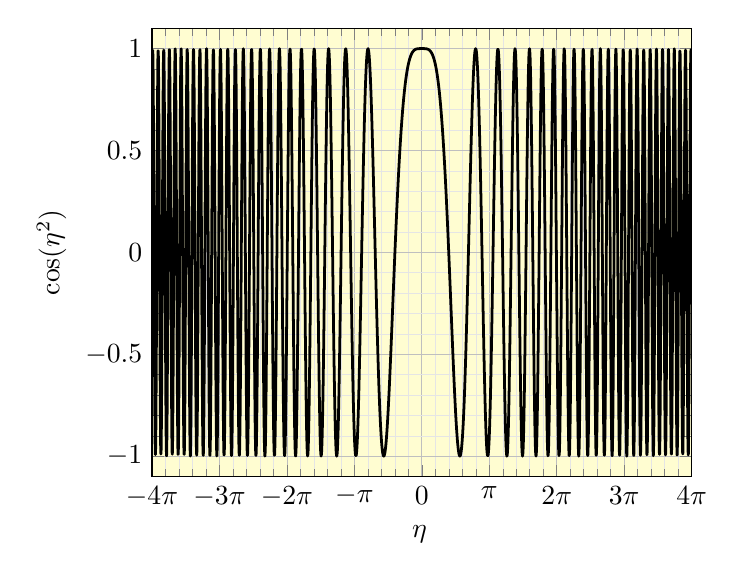
\begin{tikzpicture}[scale=1.00]
\begin{axis}[
	axis background/.style={fill=yellow!18},
	legend cell align=left,
	grid style={line width=.2pt,draw=gray!20},
	major grid style={line width=.3pt,draw=gray!50},
	grid=both,
	xlabel={$\eta$\,\si{\radian}},
	ylabel={$\cos(\eta^2)$},
	domain=-4*pi:4*pi,
	minor y tick num = 4,
	minor x tick num = 4,
	xmin=-4*pi,
	xmax=4*pi,
	ymin=-1.1,
	ymax=1.1,
        ytick={-1,-0.5,0,0.5,1},
        xtick={-4*pi,-3*pi,-2*pi,-pi,0,pi,2*pi,3*pi,4*pi},
        xticklabels={$-4\pi$,$-3\pi$,$-2\pi$,$-\pi$,$0$,$\pi$,$2\pi$,$3\pi$,$4\pi$}]
        \addplot[smooth,domain=-4*pi:4*pi,color=black,mark=none,samples=1000,line
        width=1pt,line join=round] {cos(deg(x^2)};
      \end{axis}
    \end{tikzpicture}
    \caption{Gráfica de la función $\cos(\eta^2)$. Se puede observar
      la rapidez de la oscilación en cuanto nos alejamos del punto
      $\eta = 0$.}
    \label{fig:cosx2}
  \end{figure}

  \subsubsection{Desarrollo en serie de las funciones de onda}
  Desarollamos en serie de potencias la función de onda
  $\psi(x+\eta, t)$ hasta segundo orden
  \[
    \psi(x+\eta,t)
    =
    \psi(x)
    + \eta\kern1pt\dfrac{\partial\psi}{\partial x}
    + \dfrac{1}{2}\kern1pt\eta^2 \kern1pt\dfrac{\partial^2\psi}{\partial x^2}
  \]
  
  Desarrollamos en serie de potencias la otra función de onda
  $\psi(x,t+\varepsilon)$ hasta primer orden\footnotemark
  \footnotetext{En la exponencial de la integral de la
    ecuación~(\ref{eq:funcion_onda_eta}) se encuentra el cociente
    $\eta^2/\varepsilon$; por tanto si la variable $\eta$ se
    desarrolla hasta segundo orden, $\varepsilon$ se debería
    desarrollar hasta primer orden, pues si se desarrollara hasta un
    orden mayor, la integral empezaría a oscilar muy rápidamente y los
    términos correspondientes no contribuirían a la integral en la
    práctica.}
  \[
    \psi(x,t+\varepsilon)
    =
    \psi(x,t)
    + \varepsilon\kern1pt\dfrac{\partial\psi}{\partial t}
  \]

  La ecuación~(\ref{eq:funcion_onda_eta}) queda
  \[
    \psi + \varepsilon\kern1pt\dfrac{\partial\psi}{\partial t}
    \approx
      \int_{-\infty}^{\infty}
      d\eta\, \dfrac{1}{c}\,\exp\left\{\dfrac{im}{2\hslash\varepsilon}\kern1pt \eta^2\right\}\,
      \left(\psi
      + \eta\kern1pt\dfrac{\partial\psi}{\partial x}
      + \dfrac{1}{2}\,\eta^2\kern1pt\dfrac{\partial^2\psi}{\partial x^2}\right)
  \]

\begin{align*}
   \psi + \varepsilon\kern1pt\dfrac{\partial\psi}{\partial t}
   \approx
   &\kern1pt\phantom{+} \dfrac{1}{c}\,\psi \int_{-\infty}^{\infty}
    d\eta\,\exp\left\{\dfrac{im}{2\hslash\varepsilon}\kern1pt\eta^2\right\}\\
   &+ \dfrac{1}{c}\,\dfrac{\partial\psi}{\partial x} \int_{-\infty}^{\infty}
    d\eta\,\exp\left\{\dfrac{im}{2\hslash\varepsilon}\kern1pt \eta^2\right\}\,\eta\\
   &+ \int_{-\infty}^{\infty}
    d\eta\,\dfrac{1}{c}\,\exp\left\{\dfrac{im}{2\hslash\varepsilon}\kern1pt\dfrac{1}{2}\kern1pt\eta^2\right\}\,\eta^2\kern1pt\dfrac{\partial^2\psi}{\partial x^2}
\end{align*}

Resolvemos las integrales gaussianas.
La segunda integral es nula porque es la integral entre dos límites
opuestos de una función impar.
\[
   \psi + \varepsilon\kern1pt\dfrac{\partial\psi}{\partial t}
   \approx
   \dfrac{1}{c}\psi\,\sqrt{\dfrac{\pi}{\dfrac{m}{\left(i2\hslash\varepsilon\right)}}}
   +
   0
   +
   \dfrac{1}{2c}\,\dfrac{\partial^2\psi}{\partial x^2} \dfrac{\sqrt{\pi}}{2}\,\left(\dfrac{m}{i2\hslash\varepsilon}\right)^{-3/2}
\]

\[
   \psi + \varepsilon\kern1pt\dfrac{\partial\psi}{\partial t}
   \approx
   \psi\,\dfrac{1}{c}\,\sqrt{\dfrac{i2\pi\hslash\varepsilon}{m}}
   +
   \dfrac{\sqrt{\pi}}{4}\,\dfrac{1}{c}\,\dfrac{\partial^2\psi}{\partial x^2} \left(\dfrac{i2\hslash\varepsilon}{m}\right)^{3/2}
\]

La estrategia a seguir es, primero igualar los coeficientes de $\psi$
y calcular $c$; después sustituir el valor de $c$ en los otros
sumandos que dependen de $\varepsilon$ y confiar que se puedan igualar

\begin{itemize}
\item Igualamos los coeficientes de $\psi$
\[
  1 = \dfrac{1}{c} \sqrt{\dfrac{i2\pi\hslash\varepsilon}{m}}
\]
\begin{equation}\label{eq:c}
  c = \sqrt{\dfrac{i2\pi\hslash\varepsilon}{m}}
\end{equation}

\item Sustituimos $c$ en los otros sumandos de ambos miembros
  \begin{align*}
    \varepsilon\,\dfrac{\partial\psi}{\partial t}
    &=
      \dfrac{\sqrt{\pi}}{4}\,\sqrt{\dfrac{m}{i2\pi\hslash\varepsilon}}\,\dfrac{\partial^2\psi}{\partial x^2} \left(\dfrac{i2\hslash\varepsilon}{m}\right)^{3/2}\\
    &=
      \sqrt{\dfrac{\cancelout{\pi}}{16}\,\dfrac{m}{i2\cancelout{\pi}\hslash\varepsilon}\,\dfrac{i^38\hslash^3\varepsilon^3}{m^3}}\\
  &=
    \sqrt{\dfrac{i^2\hslash^2\varepsilon^2}{4m^2}}
  \end{align*}

  Nos queda
  \[
    \varepsilon\,\dfrac{\partial\psi}{\partial t}
    =
    \varepsilon\,\dfrac{i\hslash}{2m} 
  \]

  Así
  \[
    i\hslash\dfrac{\partial\psi}{\partial t}
    =
    -\dfrac{\hslash^2}{2m}\,\dfrac{\partial^2\psi}{\partial x^2}
  \]
  que es la ecuación de Schrödinger para una partícula libre (sin $U(x)$).
\end{itemize}

\subsection{Propagador de un oscilador armónico}
Calcularemos el propagador de un oscilador armónico, partiendo de la
aproximación a segundo orden de la acción,
ecuación~(\ref{eq:accion_aprox_segundo_orden})
\[
  K(x_b,t_b;x_a,t_a)
  =
  \dfrac{1}{c^{\textsc{n}}}
  \int_{-\infty}^{\infty} \mathcal{D}z\,
  \exp\left\{\dfrac{i}{\hslash}
    \left[S^{\textsc{cl}}+\int_{t_a}^{t_b}\left(\dfrac{1}{2}m\dot{x}^2-\dfrac{1}{2}U''(x)z^2\right)\right]\right\}
\]

Discretizamos el tiempo, y como $U(x)=\frac{1}{2}m\omega^2x^2$,
entonces $U''(x) = m\omega^2$
{\small
\[
 K(x_b,t_b;x_a,t_a) =
  e^{iS^{\textsc{cl}}/\hslash}
  \dfrac{1}{c^{\textsc{n}}}\,
  \int_{-\infty}^{\infty}dz_1
  \int_{-\infty}^{\infty}dz_2
  \cdots
  \int_{-\infty}^{\infty}dz_{\textsc{n}-1}
  \exp\left\{\frac{im\varepsilon}{2\hslash}
  \sum_{n=0}^{\textsc{n}-1}
  \left[\dfrac{(z_{n+1}-z_n)^2}{\varepsilon^2}-\omega^2z_n^2
  \right]\right\}
\]
}

{\small
\begin{equation}\label{eq:propagador_integral_oscilador_armonico_epsilon}
 K(x_b,t_b;x_a,t_a) =
  e^{iS^{\textsc{cl}}/\hslash}
  \dfrac{1}{c^{\textsc{n}}}\,
  \int_{-\infty}^{\infty}dz_1
  \int_{-\infty}^{\infty}dz_2
  \cdots
  \int_{-\infty}^{\infty}dz_{\textsc{n}-1}
  \exp\left\{-\frac{m}{2i\hslash\varepsilon}
    \sum_{n=0}^{\textsc{n}-1}
    \left[(z_{n+1}-z_n)^2-\varepsilon^2\omega^2z_n^2\right]\right\}
\end{equation}
}

{\small
\begin{align*}
  \sum_{n=0}^{\textsc{n}-1} \left[(z_{n+1}-z_n)^2 - \varepsilon^2\omega^2z_n\right]
  &=
    z_1^2 + (z_2-z_1)^2 -\varepsilon^2\omega^2z_1^2
    + (z_3-z_2)^2 - \varepsilon^2\omega^2z_2^2
    + \cdots
    + z_{\textsc{n}-1}^2 - \varepsilon^2\omega^2z_{\textsc{n}-1}^2\\
  &=
    (2-\varepsilon^2\omega^2)z_1^2
    + (2-\varepsilon^2\omega^2)z_2^2
    +\cdots
    -2z_1z_2
    -2z_2z_3
    - \cdots\\
  &= \sum_{n=1}^{\textsc{n}-1}\left[(2-\varepsilon^2\omega^2)z_n^2-2z_nz_{n+1}\right]
    = \vvv{z}^\transp \mmm{M} \vvv{z}
\end{align*}
}

De manera que la integral que forma el propagador, sustituyendo además
el valor de $c$, se puede escribir
\begin{align*}
  \dfrac{1}{c^{\textsc{n}}}\,
  \int_{-\infty}^{\infty}\mathcal{D}z\,
  \exp\left\{-\frac{m}{2i\hslash\varepsilon}
  \vvv{z}^\transp \mmm{M} \vvv{z}                    
  \right\}
  &=
    \dfrac{1}{\left(\dfrac{2\pi i\hslash\varepsilon}{m}\right)^{\textsc{n}}}
    \sqrt{
    \dfrac{\pi^{\textsc{n}-1}}
    {\left(\dfrac{m}{2i\hslash\varepsilon}\right)^{\textsc{n}-1}}\,
    \cdot\dfrac{1}{\det(\mmm{M})}}
\end{align*}

\begin{equation}\label{eq:integral_propagador_oscilador_armonico}
  \dfrac{1}{c^{\textsc{n}}}\,
  \int_{-\infty}^{\infty}\mathcal{D}z\,
  \exp\left\{-\frac{m}{2i\hslash\varepsilon}
  \vvv{z}^\transp \mmm{M} \vvv{z}                    
  \right\}
  =
    \sqrt{
    \dfrac{m}{2\pi i\hslash\varepsilon}
    \cdot\dfrac{1}{\det(\mmm{M})}}
\end{equation}


Nótese que el determinante de $\mmm{M}$ no vale $N$, como en el caso
del propagador de una partícula libre, porque $U''(x)\neq 0$.

La matriz $\mmm{M}$ es
\begin{equation}\label{eq:matriz_propagador_oscilador_armonico}
  \mmm{M}
  =
  \begin{pmatrix}
    2-\varepsilon^2\omega^2 & -1 & 0 & 0 & \dots & 0 \\
    -1 & 2-\varepsilon^2\omega^2 & -1  & 0 & \dots & 0 \\
    0 & -1 & 2-\varepsilon^2\omega^2 & -1  & \dots & 0 \\
    0 & 0 & -1 & 2-\varepsilon^2\omega^2 & \dots & 0 \\
    \vdots & \vdots & \vdots & \vdots & \ddots & \vdots\\
    0 & 0 & 0 & 0 & \dots & 2-\varepsilon^2\omega^2\\
  \end{pmatrix}
\end{equation}

Desarrollaremos una buena parte de la sección resolviendo el determinante
de $\mmm{M}$
\begin{equation}\label{eq:determinante_propagador_oscilador_armonico}
  \det(\mmm{M})
  =
  \begin{vmatrix}
    2-\varepsilon^2\omega^2 & -1 & 0 & 0 & \dots & 0 \\
    -1 & 2-\varepsilon^2\omega^2 & -1  & 0 & \dots & 0 \\
    0 & -1 & 2-\varepsilon^2\omega^2 & -1  & \dots & 0 \\
    0 & 0 & -1 & 2-\varepsilon^2\omega^2 & \dots & 0 \\
    \vdots & \vdots & \vdots & \vdots & \ddots & \vdots\\
    0 & 0 & 0 & 0 & \dots & 2-\varepsilon^2\omega^2\\
  \end{vmatrix}
\end{equation}

Es costumbre resolverlo utilizando desarrollo de Fourier, pero aquí lo
haremos mediante otras técnicas.

\subsubsection{Relación de recurrencia}
Nuestro primer objetivo es obtener una relación de recurrencia entre
determinantes de distinto orden. Para simplificar las expresiones
empezamos llamando $b$ a los elementos diagonales
\[
  b = 2-\varepsilon^2\omega^2
\]

Si $N=1$, entonces $n=0,1$ y el orden de la matriz es, quitando los
valores extremos, $n=N-1= 1-1 = 0$, y por defecto el determinante será
$1$
\[
  D_0 = 1
\]

Para $N=2$, $n=N-1=2-1=1$
\[
  D_1 = \begin{vmatrix}b\end{vmatrix} = b
\]

Para $N=3$, $n=N-1 = 3-1 = 2$
\[
  D_2
  =
  \begin{vmatrix}b & -1\\ -1 & b\end{vmatrix}
  = b^2 -1 = b D_1 - D_0
\]

Si $N=4$, $n=N-1 = 4-1 = 3$
\[
  D_3
  =
  \begin{vmatrix}b & -1 & 0\\ -1 & b & -1\\ 0 & -1 & b\end{vmatrix}
  = b\begin{vmatrix}b & -1\\ -1 & b\end{vmatrix}
  + \begin{vmatrix}-1 & -1\\ 0 & b\end{vmatrix}
  = b D_2 - D_1
\]

Con $N=5$, $n=N-1 = 5-1 = 4$
\[
  D_4
  =
  \begin{vmatrix}
    b & -1 & 0 & 0\\ -1 & b & -1 & 0\\ 0 & -1 & b & -1\\0&0&-1&b
  \end{vmatrix}
  = b\begin{vmatrix}b & -1&0\\ -1 & b&-1\\0&-1&b\end{vmatrix}
  + \begin{vmatrix}-1 & -1 & 0\\ 0 & -1 & -1\\0 & -1 & b\end{vmatrix}
  = \cdots = b D_3 - D_1
\]

La relación de recurrencia es
\[
  D_n = b D_{n-1} - D_{n-2}
\]

\subsubsection{Ecuación para obtener $D_n$ mediante la relación de
  recurrencia}
Para poder calcular $D_n$, se necesita una ecuación de segundo grado,
pues el mayor término es $n$ y el menor es dos números menor, $n-2$.

La ecuación auxiliar de segundo grado es
\[
  r^2 = br^1-r^0
\]
\[
  r^2-br+1 = 0
\]

Resolvemos la ecuación y obtenemos dos valores para $r$
\begin{align*}
  r_1 &= \dfrac{1}{2}\left(b+\sqrt{b^2-4}\right)\\
  r_2 &= \dfrac{1}{2}\left(b-\sqrt{b^2-4}\right)
\end{align*}

El determinante $D_n$ tendrá la forma
\[
  D_n = P_1 r_1^n + P_2 r_2^n
\]
donde $P_1$ y $P_2$ son dos polinomios de grado igual a una unidad
menor que la multiplicidad de la raíz a la que acompañan. Como la
multiplicidad de las dos raíces es $1$, ambos polinomios son de grado
cero, esto es, son dos constantes, que llamaremos $A$ y $B$. El
determinante queda
\begin{equation}\label{eq:Dn_con_A_B}
  D_n
  =
  A r_1^n + B r_2^n
\end{equation}

\subsubsection{Cálculo de las constantes $A$ y $B$}
Ahora nuestro objetivo será calcular las constantes $A$ y $B$.
Desarrollamos las soluciones sustituyendo $b$ por $=2-\varepsilon^2\omega^2$, y
como $\varepsilon$ tiende a cero, despreciaremos los términos con
$\varepsilon^2$ y superiores
\begin{align*}
  r_1
  &=
  \dfrac{1}{2}\left(
    2-\varepsilon^2\omega^2 + \sqrt{(2-\varepsilon^2\omega^2)^2-4}
    \right)
    \approx
    \dfrac{1}{2}\left(
    2
    + \sqrt{(\cancelout{4}-4\varepsilon^2\omega^2)-\cancelout{4}}
    \right)
  =
    \dfrac{1}{2}\left(
    2 + 2i\varepsilon\omega
    \right)\\
  &= 1+i\epsilon\omega
\end{align*}
De forma similar obtendríamos
\[
  r_2 \approx 1 - i\epsilon\omega
\]

Como $A$ y $B$ son constantes para cualquier valor de $n$, utilicemos
la ecuación~(\ref{eq:Dn_con_A_B}) para los valores $n=3$ y $n=4$
\begin{align*}
  D_2 &= A (1+i\varepsilon\omega)^2 + B(1-i\varepsilon\omega)^2\\
  D_3 &= A (1+i\varepsilon\omega)^3 + B(1-i\varepsilon\omega)^3
\end{align*}

Hemos de realizar varias tareas
\begin{itemize}
\item Encontrar una expresión para $D_2$ y $D_3$ cuando
  $\varepsilon \rightarrow 0$.

  Se pueden seguir varias estrategias:
  \begin{itemize}
  \item Una de ellas consiste en recordar que si $\varepsilon$ es un
    infinitésimo, el propagador de la
    ecuación~(\ref{eq:propagador_integral_oscilador_armonico_epsilon})
    tiende al de una partícula libre, por lo que
    \[
      D_n = D_{\textsc{n}-1} \approx N
    \]
    con lo que $D_2\approx 3$ y $D_3\approx 4$.

    \item
    Otra forma sería desarrollar $D_2$ y $D_3$ de las expresiones xxxxxxx.
    Por ejemplo, para $D_2$, despreciando los términos en
    $\varepsilon^2$ y superiores
    \[
      D_2 = b^2 - 1 = (2-\varepsilon^2\omega^2)^2-1
      = 4 -4\varepsilon^2\omega^2 + \varepsilon^4\omega^4 -1 
      \approx
      4 - 1
      = 3
    \]

    Para $D_3$, recordando que $D_2\approx 3$ y que $D_1= b$
    \[
      D_3
      = b D_2 - D_1
      \approx
      (2-\varepsilon^2\omega^2) 3 - (2-\varepsilon^2\omega^2)
      \approx
      6 - 2
      = 4
    \]
  \end{itemize}

\item Hay que aproximar $(1\pm i\varepsilon\omega)^2$
  \begin{align*}
    (1+i\varepsilon\omega)^2
    &\approx
    1 + 2i\varepsilon\omega\\
    (1-\varepsilon\omega)^2
    &\approx
    1 - 2i\varepsilon\omega
  \end{align*}

\item Hay que aproximar $(1\pm i\varepsilon\omega)^3$
  \begin{align*}
    (1+i\varepsilon\omega)^3
    &= (1+i\varepsilon\omega) (1+i\varepsilon\omega)^2
    \approx (1+i\varepsilon\omega) (1+2i\varepsilon\omega)
      \approx 1+3i\varepsilon\omega\\
    (1-i\varepsilon\omega)^3
    &= \cdots
    \approx
    1-3i\varepsilon\omega
  \end{align*}
\end{itemize}

Las expresiones aproximadas para $D_2$ y $D_3$, para resolver $A$ y $B$ son
  \begin{align*}
    3 &= A\kern1pt (1+2i\varepsilon\omega) + B\kern1pt (1-2i\varepsilon\omega)\\
    4 &= A\kern1pt (1+3i\varepsilon\omega) + B\kern1pt (1-3i\varepsilon\omega)
  \end{align*}


  Resolvemos mediante cálculo matricial
  $\vvv{n} = \mmm{M} \vvv{c}$
  
  \[
    \begin{pmatrix}3 \\ 4\end{pmatrix}
    =
    \begin{pmatrix}
      1+2i\varepsilon\omega & 1-2i\varepsilon\omega\\
      1+3i\varepsilon\omega & 1-3i\varepsilon\omega
    \end{pmatrix}
    \begin{pmatrix}A \\ B\end{pmatrix}
  \]

  Necesitamos el determinante de la matriz para hallar su inversa
  \begin{align*}
    \det(M)
    &=
      \begin{vmatrix}
      1+2i\varepsilon\omega & 1-2i\varepsilon\omega\\
      1+3i\varepsilon\omega & 1-3i\varepsilon\omega
    \end{vmatrix}
    =
    (1+2i\varepsilon\omega)(1-3i\varepsilon\omega)
    - (1-2i\varepsilon\omega) (1+3i\varepsilon\omega)\\
    &\approx
      (1-3i\varepsilon\omega+2i\varepsilon\omega)
      - (1+3i\varepsilon\omega-2i\varepsilon\omega)
    = -2i\varepsilon\omega
  \end{align*}
  
  Entonces, $\vvv{c} = \mmm{M}^{-1}\vvv{n}$
  \begin{align*}
   \begin{pmatrix}A \\ B\end{pmatrix}
    &=
    \begin{pmatrix}
      1+2i\varepsilon\omega & 1-2i\varepsilon\omega\\
      1+3i\varepsilon\omega & 1-3i\varepsilon\omega
    \end{pmatrix}^{-1}
    \begin{pmatrix}3 \\ 4\end{pmatrix}
    =
    \dfrac{1}{-2i\varepsilon\omega}
    \begin{pmatrix}
      1-3i\varepsilon\omega & -1+2i\varepsilon\omega\\
      -1-3i\varepsilon\omega & 1+2i\varepsilon\omega
    \end{pmatrix}
    \begin{pmatrix}3 \\ 4\end{pmatrix}\\
    &=
      \dfrac{1}{-2i\varepsilon\omega}
      \begin{pmatrix}
        3 -9i\varepsilon\omega-4+8i\varepsilon\omega\\
        -3-9i\varepsilon\omega+4+8i\varepsilon\omega
      \end{pmatrix}
    =
      \dfrac{1}{-2i\varepsilon\omega}
      \begin{pmatrix}
        -1-i\varepsilon\omega\\
        1-i\varepsilon\omega
        \end{pmatrix}
  \end{align*}

  Los valores de $A$ y $B$ son
  \begin{align*}
    A
    &=
      \dfrac{-1-i\varepsilon\omega}{-2i\varepsilon\omega}
      =
      \dfrac{1}{2} - \dfrac{i}{2\varepsilon\omega}\\
    B
    &=
      \dfrac{1-i\varepsilon\omega}{-2i\varepsilon\omega}
      =
      \dfrac{1}{2} + \dfrac{i}{2\varepsilon\omega}
  \end{align*}

  El determinante queda
  \begin{align*}
    D_n
    &=
    \left(\dfrac{1}{2}-\dfrac{i}{2\varepsilon\omega}\right)(1+i\varepsilon\omega)^n
    +
      \left(\dfrac{1}{2}+\dfrac{i}{2\varepsilon\omega}\right)(1-i\varepsilon\omega)^n
  \end{align*}

  Calculamos el límite de $(1\pm i\varepsilon\omega)^n$ cuando $N$
  tiende a infinito
  \[
    \lim_{\textsc{n}\to\infty}(1+i\varepsilon\omega)^n
    =
    \left[1+\dfrac{i\omega(t_b-t_a)}{N}\right]^{N-1}
    \approx
    \left[1+\dfrac{i\omega(t_b-t_a)}{N}\right]^N
    =
    e^{i\omega (t_b-t_a)}
  \]
  \[
    \lim_{\textsc{n}\to\infty}(1-i\varepsilon\omega)^n
    =
    \left[1-\dfrac{i\omega(t_b-t_a)}{N}\right]^{N-1}
    \approx
    \left[1+\dfrac{-i\omega(t_b-t_a)}{N}\right]^N
    =
    e^{-i\omega (t_b-t_a)}
  \]

  Reescribimos el determinante en una parte que no depende de
  $\varepsilon$ y otra que sí
  
\begin{align*}
    D_n
    &=
    \left(\dfrac{1}{2}-\dfrac{i}{2\varepsilon\omega}\right)\,e^{i\omega\kern1pt(t_b-t_a)}
    +
    \left(\dfrac{1}{2}+\dfrac{i}{2\varepsilon\omega}\right)e^{-i\omega\kern1pt(t_b-t_a)}\\
    &=\dfrac{1}{2}\left[e^{i\omega\kern1pt(t_b-t_a)}+e^{-i\omega\kern1pt(t_b-t_a)}\right]
      + \dfrac{i}{2\varepsilon\omega}\left[e^{-i\omega\kern1pt(t_b-t_a)}-e^{i\omega\kern1pt(t_b-t_a)}\right]\\
    &=
      L - \dfrac{i}{2\varepsilon\omega}\,2i\sin\omega(t_b-t_a)
    = L + \dfrac{\sin\omega(t_b-t_a)}{\varepsilon\omega}
\end{align*}
donde hemos llamado $L$ a la parte acotada, que no depende de $\varepsilon$.

Recordamos la integral del propagador del oscilador armónico,
ecuación~(\ref{eq:integral_propagador_oscilador_armonico})
{\small
\begin{align*}
  \dfrac{1}{c^{\textsc{n}}}\,
  \int_{-\infty}^{\infty}\mathcal{D}z\,
  \exp\left\{-\frac{m}{2i\hslash\varepsilon}
  \vvv{z}^\transp \mmm{M} \vvv{z}                    
  \right\}
  &=
    \sqrt{
    \dfrac{m}{2\pi i\hslash\varepsilon}
    \cdot\dfrac{1}{\det(\mmm{M})}}
  =
    \sqrt{
    \dfrac{m}{2\pi i\hslash\varepsilon}
    \cdot\dfrac{1}
    {
    L+\dfrac{\sin\omega(t_b-t_a)}{\varepsilon\omega}
    }}\\
  &=
    \sqrt{
    \dfrac{m}
    {
    2\pi i\hslash\varepsilon L
    +
    \dfrac{2\pi i\hslash\cancelout{\varepsilon}\sin\omega(t_b-t_a)}
    {\cancelout{\varepsilon}\omega}
    }}    
\end{align*}
}

En el límite, cuando $\varepsilon$ tiende a cero, desaparece el término con $L$
\begin{align*}
  \dfrac{1}{c^{\textsc{n}}}\,
  \int_{-\infty}^{\infty}\mathcal{D}z\,
  \exp\left\{-\frac{m}{2i\hslash\varepsilon}
  \vvv{z}^\transp \mmm{M} \vvv{z}                    
  \right\}
  &=
    \sqrt{
    \dfrac{m\omega}
    {
    2\pi i\hslash\sin\omega(t_b-t_a)}
    }
\end{align*}

El propagador del oscilador armónico queda, utilizando la expresión de
la acción clásica de un oscilador armónico,
ecuación~(\ref{eq:oscilador_armonico_accion_clasica})
{\small
  \begin{equation}\label{eq:propagador_oscilador_armonico}
    K(x_b,t_b;x_a,t_a) =
      \sqrt{
    \dfrac{m\omega}
    {
    2\pi i\hslash\sin\omega(t_b-t_a)}
    }    
  \exp\left\{
    \dfrac{m\omega}
    {2\sin\omega(t_b-t_a)}\,
    \left[(x_a^2+x_b^2)\,\cos\omega(t_b-t_a) - 2x_ax_b\right]
  \right\}
\end{equation}
}



%%% Local Variables:
%%% mode: latex
%%% TeX-engine: luatex
%%% TeX-master: "../mcfeynman.tex"
%%% End:


% -----------------------------------------------------------------------------
% Apéndices

%% \part{Apéndices}
%\appendix
%\clearpage
%\addappheadtotoc
%\appendixpage
%\include{./apendices/rf-coord_esfericas}
%\include{./apendices/rf-desigualdades_vectoriales}

% -----------------------------------------------------------------------------

\end{document}


%%% Local Variables:
%%% coding: utf-8
%%% mode: latex
%%% TeX-engine: luatex
%%% TeX-master: t
%%% End:
